% ============================================================================
% THE FABRIC OF BEING: an illustrated ontology of Unitary Holonomic Monism
% A popular encyclopedia-book: minimum mathematics, maximum meaning.
% Compile with pdflatex.
% ============================================================================

\documentclass[11pt,letterpaper]{article}

% === PACKAGES ===
\usepackage[utf8]{inputenc}
\usepackage[T1]{fontenc}
\usepackage{amsmath,amssymb}
\usepackage{tikz}
\usetikzlibrary{arrows.meta, positioning, calc, decorations.pathmorphing, shapes.geometric, backgrounds}
\usepackage{xcolor}
\usepackage{booktabs}
\usepackage{hyperref}
\usepackage{geometry}
\geometry{margin=1in}
\usepackage{enumitem}
\usepackage{caption}
\usepackage{tcolorbox}
\tcbuselibrary{skins,breakable}
\usepackage{float}
\usepackage{xspace}
\usepackage[protrusion=true,expansion=true]{microtype}
\usepackage{fancyhdr}
\setlength{\headheight}{14pt}
\pagestyle{fancy}
\fancyhf{}
\fancyhead[L]{\footnotesize\scshape The Fabric of Being}
\fancyhead[R]{\footnotesize\thepage}
\renewcommand{\headrulewidth}{0.2pt}
\renewcommand{\footrulewidth}{0pt}

% === COLORS === (house palette: restrained, near-white grounds, one accent per voice)
\definecolor{plosblue}{HTML}{2563AE}
\definecolor{plosgray}{HTML}{566270}
\definecolor{ember}{HTML}{A8650B}      % campfire amber
\definecolor{leaf}{HTML}{136B44}       % question green
\definecolor{fact}{HTML}{1F4E79}       % precision blue
\definecolor{softsun}{HTML}{FCF8F2}
\definecolor{softsky}{HTML}{F4F8FB}
\definecolor{softleaf}{HTML}{F3F9F5}
\definecolor{dusk}{HTML}{5D4788}
% seven voices (dimension colors)
\definecolor{cA}{HTML}{C0392B} % Articulation
\definecolor{cS}{HTML}{CA6F1E} % Structure
\definecolor{cD}{HTML}{B7950B} % Dynamics
\definecolor{cL}{HTML}{1E8449} % Logic
\definecolor{cE}{HTML}{6B4C9A} % Interiority
\definecolor{cO}{HTML}{34495E} % Ground
\definecolor{cU}{HTML}{2E86C1} % Unity

% === THE BOOK'S THREE VOICES === (house style: sharp corners, hairline frame,
%     a single weighted rule on the left, title in the frame color on the ground)
\newtcolorbox{talebox}[1][]{enhanced, colback=softsun, colframe=ember!80!black,
  coltitle=ember!70!black, colbacktitle=softsun, titlerule=0mm,
  fonttitle=\bfseries\itshape, title={#1}, boxrule=0.3pt, leftrule=2.2pt,
  arc=0pt, breakable, left=8pt, right=8pt, toptitle=3pt, bottomtitle=1pt}
\newtcolorbox{factbox}[1][]{enhanced, colback=softsky, colframe=fact,
  coltitle=fact, colbacktitle=softsky, titlerule=0mm,
  fonttitle=\bfseries, title={#1}, boxrule=0.3pt, leftrule=2.2pt,
  arc=0pt, breakable, left=8pt, right=8pt, toptitle=3pt, bottomtitle=1pt}
\newtcolorbox{askbox}[1][]{enhanced, colback=softleaf, colframe=leaf,
  coltitle=leaf!85!black, colbacktitle=softleaf, titlerule=0mm,
  fonttitle=\bfseries, title={#1}, boxrule=0.3pt, leftrule=2.2pt,
  arc=0pt, breakable, left=8pt, right=8pt, toptitle=3pt, bottomtitle=1pt}

% === COMMANDS ===
\newcommand{\Gam}{\Gamma}
\newcommand{\stT}{\textbf{[T]}\xspace}
\newcommand{\stC}{\textbf{[C]}\xspace}
\newcommand{\stP}{\textbf{[P]}\xspace}
\newcommand{\stI}{\textbf{[I]}\xspace}
\newcommand{\stH}{\textbf{[H]}\xspace}
\newcommand{\holonsh}{\href{https://holon.sh}{holon.sh}\xspace}


% === PART THRESHOLD ===
\newcommand{\partline}[2]{%
  \clearpage\vspace*{4pt}\begin{center}
  {\color{fact}\rule{0.55\textwidth}{0.4pt}}\\[9pt]
  {\large\bfseries #1}\\[7pt]
  \begin{minipage}{0.82\textwidth}\centering\small\itshape\color{plosgray} #2\end{minipage}\\[9pt]
  {\color{fact}\rule{0.55\textwidth}{0.4pt}}
  \end{center}\bigskip}

% === HOUSE GLYPH: the rose of seven voices ===
% \voicerose{x}{y}{radius}{dot}: colored rose at (x,y)
\newcommand{\voicerose}[4]{%
  \foreach \vang/\vcol in {90/cA,141.4/cS,192.8/cD,244.3/cL,295.7/cE,347.1/cO,38.6/cU}{%
    \draw[\vcol!55, thick] (#1,#2) -- ($(#1,#2)+(\vang:#3)$);
    \fill[\vcol] ($(#1,#2)+(\vang:#3)$) circle (#4);}}
% \voiceroseneutral{x}{y}{radius}{dot}: quiet rose for population figures
\newcommand{\voiceroseneutral}[4]{%
  \foreach \vang in {90,141.4,192.8,244.3,295.7,347.1,38.6}{%
    \draw[plosgray!40] (#1,#2) -- ($(#1,#2)+(\vang:#3)$);
    \fill[plosblue!65] ($(#1,#2)+(\vang:#3)$) circle (#4);}}

\hypersetup{colorlinks=true, linkcolor=fact, urlcolor=plosblue, citecolor=plosgray,
  pdftitle={The Fabric of Being: An Illustrated Ontology of Unitary Holonomic Monism},
  pdfauthor={The UHM corpus (holon.sh)},
  pdfsubject={Popular ontology of UHM: a mathematical optics and coherence cybernetics},
  pdfkeywords={UHM, ontology, consciousness, qualia, coherence, Fano plane, octonions}}
\captionsetup{font=small, labelfont={bf,color=fact}}

\begin{document}

% ============================= TITLE =============================
\begin{titlepage}
\centering
\vspace*{28pt}
{\Huge\bfseries The Fabric of Being}\\[10pt]
{\LARGE An Illustrated Ontology\\[3pt] of Unitary Holonomic Monism}\\[26pt]
% --- title mandala of the seven voices ---
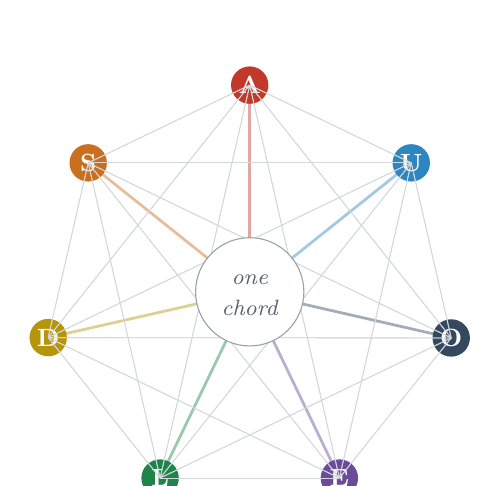
\begin{tikzpicture}[scale=1.25]
  \foreach \ang/\col/\lab in {90/cA/A, 141.4/cS/S, 192.8/cD/D, 244.3/cL/L, 295.7/cE/E, 347.1/cO/O, 38.6/cU/U}{
    \draw[\col!45, line width=1pt] (0,0) -- (\ang:2.1);
    \fill[\col] (\ang:2.1) circle (0.19);
    \node[font=\small\bfseries, text=white] at (\ang:2.1) {\lab};
  }
  \foreach \a in {90, 141.4, 192.8, 244.3, 295.7, 347.1, 38.6}{
    \foreach \b in {90, 141.4, 192.8, 244.3, 295.7, 347.1, 38.6}{
      \draw[plosgray!25, line width=0.3pt] (\a:2.1) -- (\b:2.1);
    }}
  \fill[white] (0,0) circle (0.55);
  \draw[plosgray!60] (0,0) circle (0.55);
  \node[font=\footnotesize\itshape, text=plosgray] at (0,0.12) {one};
  \node[font=\footnotesize\itshape, text=plosgray] at (0,-0.16) {chord};
\end{tikzpicture}\\[26pt]
{\large An axiomatic optics for research and practice ---\\
for every field where something lives, thinks, or is built}\\[18pt]
{\small\color{plosgray} After the theory of UHM (\holonsh) --- with honest marks\\
for what is proved, what is assumed, and what is merely beautiful so far}\\[10pt]
{\small\color{plosgray} First edition --- August 2026}
\vfill
\begin{talebox}[How to read this book]
This book speaks in three voices. \textcolor{ember}{\textbf{Amber boxes}} are
the campfire tale: images you can read to a child.
\textcolor{fact}{\textbf{Blue boxes}} are ``to be precise'': what the theory
actually claims, unadorned. \textcolor{leaf}{\textbf{Green boxes}} are
questions worth arguing about over dinner. The main text is for everyone else
--- engineers, physicians, philosophers, psychologists --- adults who want the
substance without the formulas. There are almost no formulas here; where a
number matters, it appears as a character in the story, not as an equation.
\end{talebox}
\end{titlepage}

\tableofcontents
\newpage

% ============================= HONESTY LEGEND =============================
\section*{Five marks of honesty}
\addcontentsline{toc}{section}{Five marks of honesty}

Science differs from myth not by lacking beauty but by the habit of
marking what exactly it knows. Five marks recur throughout the book:

\begin{center}
\begin{tabular}{@{}cl@{}}
\toprule
\stT & \textbf{proved}: a theorem within the theory; only the axioms are left to dispute \\
\stC & \textbf{proved conditionally}: true if the named premise holds \\
\stH & \textbf{hypothesis}: plausible, proof being sought \\
\stP & \textbf{postulate}: taken as a starting point, not derived \\
\stI & \textbf{interpretation}: a reading, not a fact; beautiful but not binding \\
\bottomrule
\end{tabular}
\end{center}

Whenever the book says ``the world is arranged thus,'' a mark stands
nearby. This is the chief difference between this encyclopedia and
sacred books: it tells you \emph{how to check that it is wrong}
(chapter~\ref{sec:check}).

Behind the five marks stands one law. A claim is \textbf{mature}
when it honors three obligations at once: it \emph{shows how it is
built} --- a concrete construction, not a promise of existence; it
\emph{submits to mechanical check} --- a machine can verify it,
with no appeal to authority or intuition; and it \emph{works} ---
there is a running representation: a program, a procedure, an
instrument. The marks are compressed fingerprints of the three:
\stT{} is all three at once; \stC{} --- all three under named
premises; \stH{} --- a formulation with a plan but no proof yet;
\stP{} --- a load-bearing assumption declared as such; \stI{} --- a
reading, kept counted and in plain sight.

Why so strict? Because knowledge meant to outlive its makers faces
three erosions: words drift, instruments change, and registers blur
--- claims, hopes, and rhetoric become indistinguishable. The three
obligations are the protection against all three at once:
constructions survive translation, mechanical checks survive
re-tooling, marked registers survive the drift of style. Hence one
house rule, felt on every page: \textbf{there are no unmarked
claims in this book}. Whatever could not carry its mark was
completed until it could, honestly demoted --- or removed. What you
are reading is what survived.

% ============================= WHAT THIS IS =============================
\section*{What you are holding: an optics, not a doctrine}
\addcontentsline{toc}{section}{What you are holding: an optics, not a doctrine}

The most useful way to hold UHM is not as ``one more picture of the
world'' but as a \textbf{mathematical optics}: a single rigorously
derived object --- seven voices, their friendships, one law of
change --- through which everything else is brought into focus in
turn: particles and space, life and death, feeling and word, family
and civilization. An optics differs from a doctrine in two ways. It
is \emph{derived}, not preached: why the lens has exactly seven
elements is a theorem, not a taste (chapter~\ref{sec:seven}). And it
\emph{focuses}: every notion in this book --- gatheredness, reserve,
coupling, color, the stress of a voice --- is not a metaphor but a
computable quantity with a threshold; a world read through this
optics acquires instrument panels (chapter~\ref{sec:health}) and
passports (chapter~\ref{sec:qualia}).

Out of the optics grows a rethinking of life that the corpus calls
\textbf{coherence cybernetics}: to live is to hold the agreement of
seven voices on supply (chapter~\ref{sec:life}); to care is to
restore flow without dimming another's floors
(chapter~\ref{sec:health}); ethics stops being a list of
prohibitions and becomes an engineering of agreements --- with
theorems where good wishes used to stand: connection adds being
(chapter~\ref{sec:others}), superintelligence grows as a forest,
not a tower (chapter~\ref{sec:society}).

And one last thing separates a working optics from a beautiful
hypothesis: it is already worked \emph{with}. The ``machine
checked'' verdicts of this book are trials of one and the same
living machinery: a working cognitive architecture has been grown
on this very seven, and the chapters on golden paths, language, and
colors retell its measurements, not thought experiments. Its
construction is not this book's subject; the fact is the subject:
the optics is strict enough to bear the weight of machines. That is
not a test of predictions about nature --- those are gathered in
the registry (chapter~\ref{sec:check}); it is a test of the
vocabulary's fitness. For a scientist or an engineer this is the
theory's chief gift: a language in which the living can not only be
spoken about --- but built.

Taken together, this makes UHM not a worldview to adopt but an
\textbf{axiomatic research programme} to work in: a hard core ---
one axiom of coupling, seven forced dimensions, theorems a machine
has checked, constants a laptop can recompute --- and around it a
widening belt of applications, each carrying its own mark and its
own way to fail. The book is built as one road through that
programme, in four movements. First the \emph{world}: what the
fabric is and why its alphabet has exactly seven letters. Then
\emph{within}: how life, the window of consciousness, the floors of
reflection and the colors of experience ignite on that fabric. Then
the \emph{pattern in action}: freedom, bold paths, language,
memory --- the mechanics of a life that acts. And finally
\emph{together and what now}: others, societies, care, death, the
observer --- ending not in a summary but in a working programme:
what this optics puts on the desk of a physicist, a physician, an
engineer of minds, a teacher --- and where it is currently
vulnerable. Whatever your field, the intended experience of this
book is the same: somewhere in these chapters your own hardest
question should suddenly appear --- restated in a language where it
can be computed, checked, or honestly marked open.

\partline{PART ONE \;\textperiodcentered\; THE WORLD}{What everything is woven of: the chord
of seven voices, the forcedness of the seven, the birth of time, of the beginning, of space and
things. Here the stage is built --- and no one is on it yet.}
\addcontentsline{toc}{section}{PART ONE · THE WORLD}

% ============================= 1. WHAT EVERYTHING IS MADE OF =============================
\section{What everything is made of}
\label{sec:fabric}

Ask a physicist of the last century what the world is made of, and the
answer is: little bricks --- particles. Ask UHM, and the answer is
different and unexpectedly musical: \emph{the world is made of
agreement}. Not of things, but of the way things hold on to one
another.

Picture seven voices singing one chord. Remove the singers and keep
\emph{the chord itself} --- the relation of pitches, the mutual tuning,
the tremble of consonant tones. In UHM this is what comes first: not
``what sounds'' but ``how it is agreed.'' Mathematicians call such an
object a density matrix and write $\Gam$: its seven diagonal cells
are the strengths of the seven voices, and the twenty-one cells above
the diagonal are their pairwise friendships (coherences). We shall
call it the \textbf{chord of the world}.

The chord has seven voices --- seven dimensions of all existence:

\begin{center}
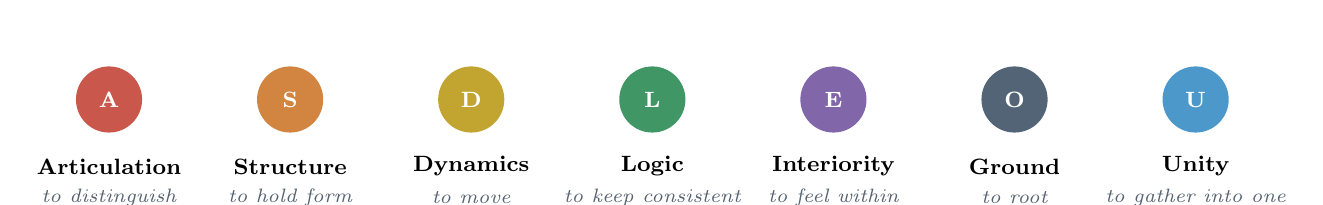
\begin{tikzpicture}[font=\small]
  \foreach \x/\col/\ltr/\name/\verb in {0/cA/A/Articulation/{to distinguish}, 2.3/cS/S/Structure/{to hold form},
    4.6/cD/D/Dynamics/{to move}, 6.9/cL/L/Logic/{to keep consistent}, 9.2/cE/E/Interiority/{to feel within},
    11.5/cO/O/Ground/{to root}, 13.8/cU/U/Unity/{to gather into one}}{
    \fill[\col!85] (\x,0) circle (0.42);
    \node[font=\footnotesize\bfseries, text=white] at (\x,0) {\ltr};
    \node[font=\footnotesize\bfseries] at (\x,-0.85) {\name};
    \node[font=\scriptsize\itshape, text=plosgray] at (\x,-1.25) {\verb};
  }
\end{tikzpicture}
\end{center}

To distinguish, to hold form, to move, to keep consistent, to feel
within, to root, to gather into one. Behind each word stands a
rigorous quantity of the theory's corpus: Articulation (A) --- the
activity of distinguishing; Structure (S) --- the stability of form;
Dynamics (D) --- the activity of process; Logic (L) --- internal
consistency; Interiority (E) --- the intensity of the inner side;
Ground (O) --- the connection to the source; Unity (U) ---
integration into a whole. This is neither a list of organs nor poetic
license:
we shall see that seven is not the author's choice but mathematics'
forced answer (chapter~\ref{sec:seven}).

\begin{talebox}[The campfire tale --- the orchestra without musicians]
Once there was an orchestra with no musicians in it. There were only
\emph{friendships between notes}: this note leans toward that one,
that one argues with a third, and together they hold one long chord.
When the friendships are strong, the chord rings --- and a thing
appears in the world: a stone, a cat, you. When the friendships tear,
the chord crumbles into rustle, and the thing dissolves. The world is
not a warehouse of bricks. The world is an orchestra of friendships.
\end{talebox}

\begin{factbox}[To be precise]
The primitive object of UHM is neither particle nor field but the
state of seven interrelated dimensions (a $7{\times}7$ density
matrix $\Gam$) together with a single law of its change. Everything
else --- particles, space, time, life, consciousness --- is
\emph{derived} as patterns of this object. Status: the seven and the
law are theorems inside the axiomatics \stT; the choice of axioms is a
postulate \stP.
\end{factbox}

\begin{askbox}[Ask yourself]
Which is ``more real'': a violin --- or the tuning in which it sounds
with the others? If you were not a body but the agreement of your
parts, what would change in how you treat yourself?
\end{askbox}

% ============================= 2. WHY SEVEN =============================
\section{Why exactly seven}
\label{sec:seven}

The number seven in this book is neither magic nor taste. Four
independent roads lead to it, and all four end at the same door.

\begin{figure}[H]
\centering
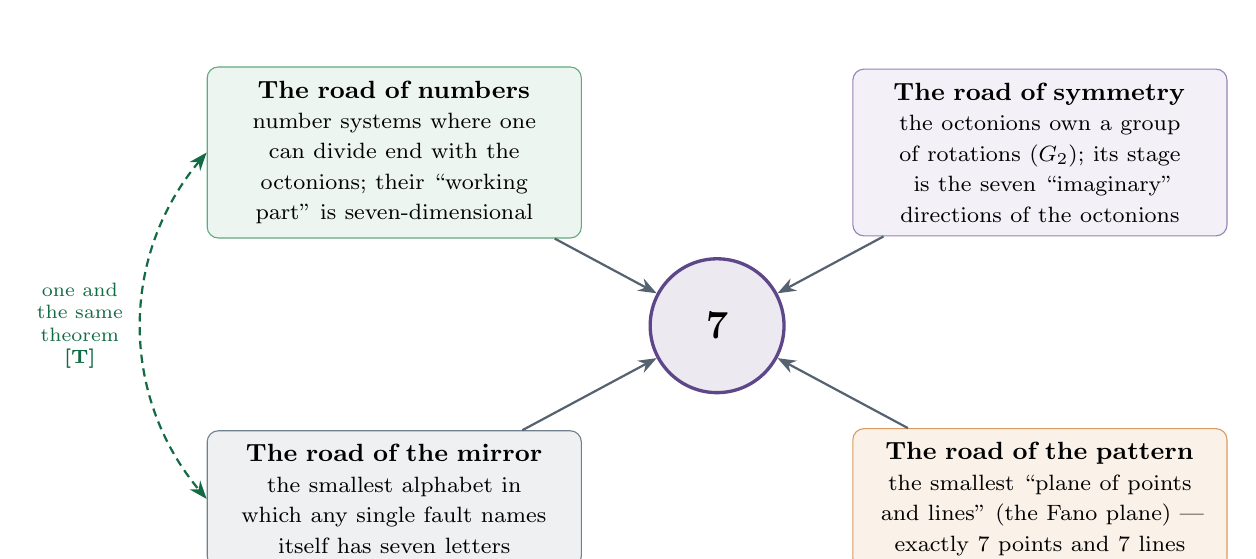
\begin{tikzpicture}[font=\small, >=Stealth]
  \node[draw=cL!70, fill=cL!8, rounded corners, text width=44mm, align=center, inner sep=5pt] (r1) at (-4.1,2.2)
    {\textbf{The road of numbers}\\ \footnotesize number systems where one can divide end with the octonions; their ``working part'' is seven-dimensional};
  \node[draw=cE!70, fill=cE!8, rounded corners, text width=44mm, align=center, inner sep=5pt] (r2) at (4.1,2.2)
    {\textbf{The road of symmetry}\\ \footnotesize the octonions own a group of rotations ($G_2$); its stage is the seven ``imaginary'' directions of the octonions};
  \node[draw=cO!70, fill=cO!8, rounded corners, text width=44mm, align=center, inner sep=5pt] (r4) at (-4.1,-2.2)
    {\textbf{The road of the mirror}\\ \footnotesize the smallest alphabet in which any single fault names itself has seven letters};
  \node[draw=cS!70, fill=cS!10, rounded corners, text width=44mm, align=center, inner sep=5pt] (r3) at (4.1,-2.2)
    {\textbf{The road of the pattern}\\ \footnotesize the smallest ``plane of points and lines'' (the Fano plane) --- exactly 7 points and 7 lines};
  \node[circle, draw=dusk, fill=dusk!12, very thick, minimum size=17mm, font=\Large\bfseries] (seven) at (0,0) {7};
  \draw[->, thick, plosgray] (r1)--(seven);
  \draw[->, thick, plosgray] (r2)--(seven);
  \draw[->, thick, plosgray] (r3)--(seven);
  \draw[->, thick, plosgray] (r4)--(seven);
  \draw[<->, densely dashed, leaf, thick] (r1.west) to[bend right=40]
    node[pos=0.5, left=3pt, font=\scriptsize, text=leaf, align=center]{one and\\ the same\\ theorem\\ \stT} (r4.west);
\end{tikzpicture}
\caption{Four roads to seven. Especially beautiful: the road of
numbers and the road of the mirror are not a coincidence but a proven
identity \stT: ``the last system where division works'' and ``the last
alphabet that checks itself'' are \emph{one and the same} property,
seen from two sides.}
\label{fig:seven}
\end{figure}

The seven voices are not wired at random: their friendships are laid
out along the seven ``lines'' of the Fano plane --- three voices to a
line, every pair of voices on exactly one line. This is the world's
\textbf{alphabet of connection}: who forms a triad with whom. The same
scheme, independently rediscovered by humans in coding theory, can
locate any single error --- which is why a world woven on Fano
\emph{can notice its own faults}. Remember this: it returns in the
chapter on life.

\begin{talebox}[The campfire tale --- seven dwarfs and the map of friendships]
Seven dwarfs owned a map: seven cottages and seven paths, three
cottages on every path. The dwarfs noticed something strange: whenever
one of them fell ill, the paths \emph{themselves} showed who it was
--- by which of them began to creak. ``Our map knows how to
complain,'' said the dwarfs. And the wise dwarf added: ``That is why
there are seven of us. Were we six or eight, the map would stay
silent, or lie.''
\end{talebox}

\begin{askbox}[Ask yourself]
Why is a ``self-checking alphabet'' a useful property for anything
alive? Imagine a creature whose faults never name themselves --- what
happens to it?
\end{askbox}

% ============================= 2b. NUMBERS =============================
\section{Why the numbers are what they are: a ladder of four worlds}
\label{sec:numbers}

Before going further, it is worth asking about the instrument itself.
The world in this book is described by numbers --- ordinary ones,
complex ones, and that famous seven of imaginary directions. But where
did \emph{the numbers themselves} come from? Why does the universe get
exactly this counting instrument and not another? UHM answers: the
instrument was not chosen --- it \emph{grew}, and the ladder of its
growth is short and breaks off by itself.

There is a simple rule --- call it the doubling rule: if you have a
world of numbers where you can add, multiply, and divide, you can
build a world twice as large by gluing two copies together. So from
the ordinary line $\mathbb{R}$ (one dimension) grows the plane
$\mathbb{C}$ (two); from it, the four-dimensional world of
quaternions $\mathbb{H}$; from that, the eight-dimensional world of
octonions $\mathbb{O}$, whose imaginary part is our seven. The ladder
runs $1 \to 2 \to 4 \to 8$ --- and every step charges a fee: first
order is lost (you cannot say which complex number is ``bigger''),
then commutativity of multiplication, then its grouping. And on the
next step --- the sixteen-dimensional sedenions --- something
irreparable happens: \emph{zero divisors} appear, pairs of nonzero
numbers whose product is zero. A number times a number --- and
suddenly nothing. A world with such a crack cannot carry
distinctions: in it, ``something'' can vanish without a trace. The
ladder breaks off at eight --- a theorem \stT, proved back in the
nineteenth century and re-verified in the theory's corpus by machine
enumeration.

That is why the seven of chapter~\ref{sec:seven} is not one option
among many but the \emph{last possible one}: the imaginary part of
the last living world of numbers.

\begin{figure}[H]
\centering
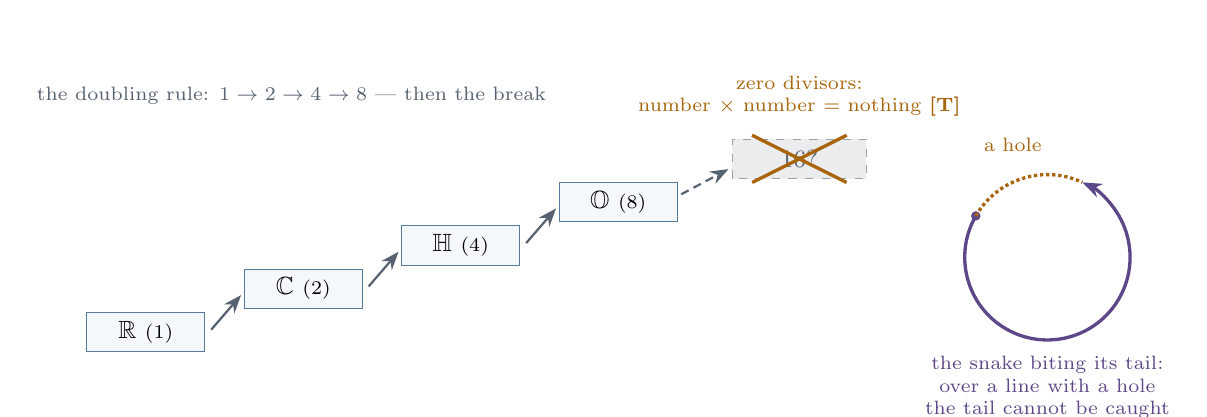
\begin{tikzpicture}[font=\small, >=Stealth]
  % ladder
  \foreach \i/\x/\lab/\dim in {0/-5.2/$\mathbb{R}$/1, 1/-3.2/$\mathbb{C}$/2, 2/-1.2/$\mathbb{H}$/4, 3/0.8/$\mathbb{O}$/8}{
    \draw[fact!75, fill=softsky] (\x,\i*0.55) rectangle (\x+1.5,\i*0.55+0.5);
    \node at (\x+0.75,\i*0.55+0.25) {\lab\ \scriptsize(\dim)};
  }
  \foreach \i/\x in {0/-3.62, 1/-1.62, 2/0.38}{
    \draw[->, thick, plosgray] (\x,\i*0.55+0.28) -- (\x+0.38,\i*0.55+0.72);
  }
  % the break: sedenions
  \draw[->, thick, densely dashed, plosgray] (2.35,2.0) -- (2.95,2.32);
  \draw[plosgray!60, fill=plosgray!12, dashed] (3.0,2.2) rectangle (4.7,2.7);
  \node[text=plosgray] at (3.85,2.45) {16?};
  \draw[ember, very thick] (3.25,2.15) -- (4.45,2.75);
  \draw[ember, very thick] (3.25,2.75) -- (4.45,2.15);
  \node[font=\scriptsize, text=ember, align=center] at (3.85,3.25)
    {zero divisors:\\ number $\times$ number $=$ nothing \stT};
  \node[font=\scriptsize, text=plosgray, align=center] at (-2.6,3.25)
    {the doubling rule: $1 \to 2 \to 4 \to 8$ --- then the break};
  % the ouroboros: a body with a gap, the head reaching for the tail
  \draw[dusk, very thick, -{Stealth[length=7pt]}] ($(7.0,1.2)+(150:1.05)$) arc (150:425:1.05);
  \fill[dusk] ($(7.0,1.2)+(150:1.05)$) circle (0.06);
  \draw[ember, very thick, densely dotted] ($(7.0,1.2)+(150:1.05)$) arc (150:65:1.05);
  \node[font=\scriptsize, text=ember] at ($(7.0,1.2)+(107:1.5)$) {a hole};
  \node[font=\scriptsize, text=dusk, align=center] at (7.0,-0.45)
    {the snake biting its tail:\\ over a line with a hole\\ the tail cannot be caught};
\end{tikzpicture}
\caption{Left: the ladder of number worlds. Each step is a doubling
with a fee; at sixteen, zero divisors appear --- a crack through which
distinctions vanish --- and the ladder breaks off \stT. Right: why the
number line is \emph{gapless} --- the self-model's closure (the snake
must reach its own tail) is impossible over a line with holes;
continuity is not an assumption but a consequence of the ouroboros
\stT.}
\label{fig:numbers}
\end{figure}

And this chapter holds a second, quieter miracle. Why is the number
line \emph{solid}, without holes? The corpus proves \stT{} that this
follows from the theory's most ancient image --- the snake biting its
own tail. A world that models itself (chapter~\ref{sec:observer})
must be able to \emph{reach itself}: a continuous self-mapping must
have a fixed point. Over a line with holes --- say, over fractions
alone --- the snake literally leaps past its own tail through a gap,
and the closure fails. The demand ``the snake always catches its
tail'' \emph{forces} a solid line --- and with it continuous time:
the flow of the law is well-defined because the numbers are complete.
Time runs smoothly not out of the world's habit, but because the
world holds on to itself.

\begin{talebox}[The campfire tale --- the smith and the four ingots]
A smith forged worlds for counting. The first ingot was a rod:
straight, honest, everything on it in order. The second was a sheet:
on it you could already circle. The third was a block: inside it you
could turn. The fourth was an eight-sided bell: it alone could ring
with seven voices at once. The smith swung at a fifth --- and the
ingot cracked: strike it, and there is no ring --- it swallows
itself. ``No further forging,'' said the smith, and kept the bell.
Since then everything that exists rings with seven voices.
\end{talebox}

\begin{askbox}[Ask yourself]
The doubling rule gives $1, 2, 4, 8$ --- and death at $16$. Find a
ladder in your own life that grows by doubling and somewhere breaks
off by itself: a team that still gets along; a list of tasks that
still fits in your head. What plays the role of the ``zero divisor''
--- the sign that the next step is no longer alive?
\end{askbox}

% ============================= 3. TIME =============================
\section{What time is}
\label{sec:time}

In the everyday picture, time is a river: it flows by itself, and we
float. UHM says something stricter and more interesting: \emph{there
is no river}. The total state of the world does not change at all ---
only its parts change \emph{relative to one another}. Time is not a
stage; it is a dance.

Picture two dancers with no music anywhere. Neither moves ``in time''
--- yet each moves \emph{in step with the other}. Ask the first
``what time is it,'' and he answers by glancing at the second's pose.
In UHM the role of such a partner is played by one of the seven
voices --- Ground (O): its measured ``breathing'' serves as the clock
for all the rest. The clock is not outside the world; the clock is
one of its voices.

\begin{figure}[H]
\centering
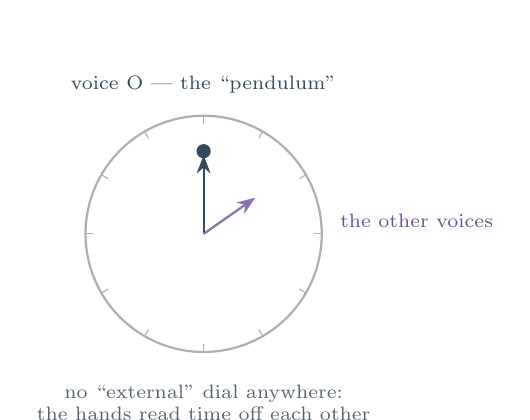
\begin{tikzpicture}[font=\small, >=Stealth]
  \draw[plosgray!50, thick] (0,0) circle (1.5);
  \foreach \a in {0,30,...,330}{\draw[plosgray!50] (\a:1.4)--(\a:1.5);}
  \fill[cO] (90:1.05) circle (0.09);
  \node[font=\scriptsize, text=cO] at (90:1.9) {voice O --- the ``pendulum''};
  \draw[->, thick, cO] (0,0)--(90:1.0);
  \draw[->, thick, cE!80] (0,0)--(35:0.8);
  \node[font=\scriptsize, text=cE, anchor=west] at (6:1.62) {the other voices};
  \node[font=\scriptsize, text=plosgray, align=center] at (0,-2.15)
    {no ``external'' dial anywhere:\\ the hands read time off each other};
\end{tikzpicture}
\caption{Time in UHM: not a river the world floats in, but the mutual
attunement of the world's parts. The question ``what was there when
time did not yet exist'' turns from a deep one into a grammatical
error --- like ``what is north of the North Pole.''}
\label{fig:time}
\end{figure}

\begin{factbox}[To be precise]
The total state of the universe is stationary; internal time arises
relative to the ``clock'' voice O (the Page--Wootters mechanism)
\stT. A consequence that matters for the next chapter: while the
voice O is not yet distinguished among the seven, the words
``earlier'' and ``later'' are not defined at all.
\end{factbox}

% ============================= 4. THE SOURCE =============================
\section{A beginning that had no ``before''}
\label{sec:source}

Now we are ready for the chief question of any ontology: \emph{how did
it all begin?} And for UHM's honest answer, which has three layers.

\textbf{Layer one --- what there was ``in the beginning'' \stP.} The
theory postulates an initial state it calls the \textbf{Source}: all
seven voices merged into one perfect note, sung with equal strength.
It is the most agreed state possible --- and at the same time the most
\emph{undifferentiated}: in it, nothing differs from anything. No
voice is distinguished --- hence (chapter~\ref{sec:time}) there is no
clock, no ``earlier,'' no ``before.'' The Source did not exist ``long
ago'' --- it is outside time, as a book's cover is outside its pages.

A beautiful strictness: the very shape of the Source is not
arbitrary. It is proved \stT{} that there exists exactly \emph{one}
state in which no voice is distinguished, and exactly \emph{one}
maximally agreed state --- and they are the same state. The Source is
unique twice over.

\textbf{Layer two --- why it all began \stT.} Here is a theorem worth
telling children: \emph{perfection is unstable}. The Source is not a
point of rest. The law of the world, applied to the perfectly merged
chord, immediately yields a nonzero push: the chord begins to
unlayer. Moreover, an amplifying loop is hidden in the law: as soon
as the voice of Interiority (E) and the voice of Ground (O) differ from
the rest even slightly, their difference begins to feed itself.
Symmetry breaks neither by chance nor by anyone's will but
\emph{inevitably} --- as a pencil balanced on its tip inevitably
falls, with this difference: here it is also proved that the ``tip''
cannot be a point of equilibrium at all.

\textbf{Layer three --- where it all went \stT.} Machine verification
of the law (it is literally integrated on a computer) shows that from
the Source the world slides not just anywhere but into a \emph{living}
state --- into the very window of viability that
chapter~\ref{sec:life} is about. Unlayering births differences,
differences birth clocks, clocks birth history. By the theory's
estimate, the first moments of that history took about seven Planck
times --- around $4\cdot10^{-43}$ seconds \stC.

\begin{figure}[H]
\centering
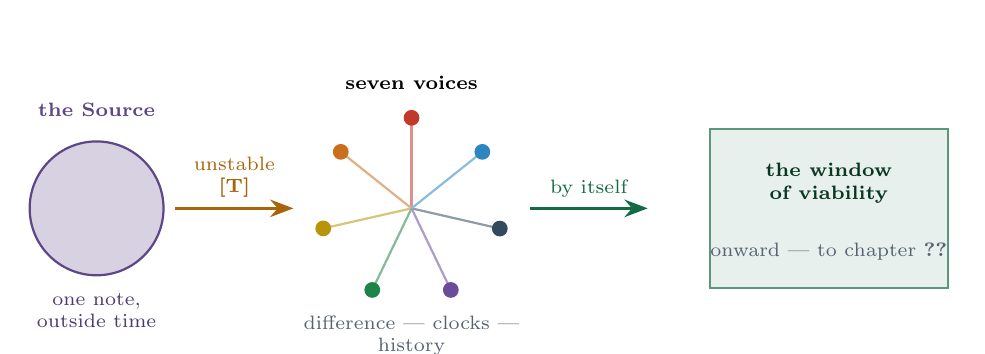
\begin{tikzpicture}[font=\small, >=Stealth]
  % Source
  \fill[dusk!25] (-5.2,0) circle (0.85);
  \draw[dusk, thick] (-5.2,0) circle (0.85);
  \node[font=\scriptsize\bfseries, text=dusk] at (-5.2,1.25) {the Source};
  \node[font=\scriptsize, text=dusk!80!black, align=center] at (-5.2,-1.3)
    {one note,\\ outside time};
  % instability arrow
  \draw[->, very thick, ember] (-4.2,0) -- (-2.7,0)
    node[midway, above, font=\scriptsize, text=ember, align=center]{unstable\\ \stT};
  % unlayering
  \voicerose{-1.2}{0}{1.15}{0.1}
  \node[font=\scriptsize\bfseries] at (-1.2,1.6) {seven voices};
  \node[font=\scriptsize, text=plosgray, align=center] at (-1.2,-1.62) {difference --- clocks ---\\ history};
  % arrow into window
  \draw[->, very thick, leaf] (0.3,0) -- (1.8,0)
    node[midway, above, font=\scriptsize, text=leaf]{by itself};
  % window of life
  \draw[leaf!70, very thick] (2.6,-1.0) rectangle (5.6,1.0);
  \fill[leaf!10] (2.6,-1.0) rectangle (5.6,1.0);
  \node[font=\scriptsize\bfseries, text=leaf!50!black, align=center] at (4.1,0.32)
    {the window\\ of viability};
  \node[font=\scriptsize, text=plosgray] at (4.1,-0.55) {onward --- to chapter~\ref{sec:life}};
\end{tikzpicture}
\caption{Cosmogenesis in UHM: the Source (postulate \stP) is unstable
(theorem \stT), unlayers into seven voices with clocks and history,
and slides \emph{by itself} into the window of life (machine
verified). The question ``what was before?'' is dissolved: ``before''
is a word born at the second step of this picture.}
\label{fig:source}
\end{figure}

\begin{talebox}[The campfire tale --- the note that grew too full]
First there was one note --- a note so even that it held no up and
no down, no yesterday and no tomorrow. But a perfect note keeps a
secret: it has nothing to lean on. It trembled --- and out of the
tremble seven voices were born. One began to count beats --- and
``earlier'' and ``later'' appeared. Another began to listen to itself
--- and ``inside'' appeared. The note did not break. The note
\emph{blossomed}, like a bud too perfect not to flower.
\end{talebox}

\begin{factbox}[The honest remainder]
What is proved here and what is not. The instability of the Source,
the amplifying loop, the slide into the living window --- theorems
and machine checks \stT. The Source itself is a postulate \stP:
``why exactly this initial state'' is an open question. The answer
``nothing is unstable because it cannot agree with itself'' is a
philosophical position \stI, not a theorem --- and the book owes you
that sentence out loud.
\end{factbox}

\begin{askbox}[Ask yourself]
``Perfection is unstable'' --- where have you met this in life? A
blank page, ideal silence, a ``perfect'' relationship without a
single argument\ldots{} What do these instabilities share with the
Source?
\end{askbox}

% ============================= 4b. THE STAGE =============================
\section{The stage: why space is three-dimensional}
\label{sec:space}

We are used to thinking that things sit \emph{in} space, like
furniture in a room. UHM turns the picture around: \textbf{space sits
in things} --- it is not a box the world was put into, but the way a
part of the voices holds one another.

Recall the unlayering of the Source (chapter~\ref{sec:source}). Once
the voice of Ground (O) became the clock, what remains of the choir
of all the world's rotations is the sub-choir that \emph{spares the
clock} --- and its smallest stage has exactly \textbf{three}
independent directions: a theorem \stT, pure mathematics of the
seven. That is the whole secret of length, width, and height. The six
non-clock voices meanwhile split into two triples: an outward one,
whose directions unfold into familiar distance, and an inward one,
whose directions are curled into microscopic rings and are felt not
as ``places'' but as the inner properties of particles. Which voices
face outward --- the theory points to Articulation, Structure, and
Dynamics --- and which inward (Logic, Interiority, Unity) is an
identification under one physical hypothesis \stC; the number of
axes itself does not depend on it.

Better still: the stage has an arrow. One time direction and three
space directions --- the famous $(1{,}3)$ signature of our world ---
is derived, not postulated: time inherits its sign from the clock
voice O, space from the outward triple \stT{} (the last step under
one technical condition of physical honesty \stC). Even the fact
that the world has a ``forward'' and a ``wide'' follows from the
same seven.

\begin{figure}[H]
\centering
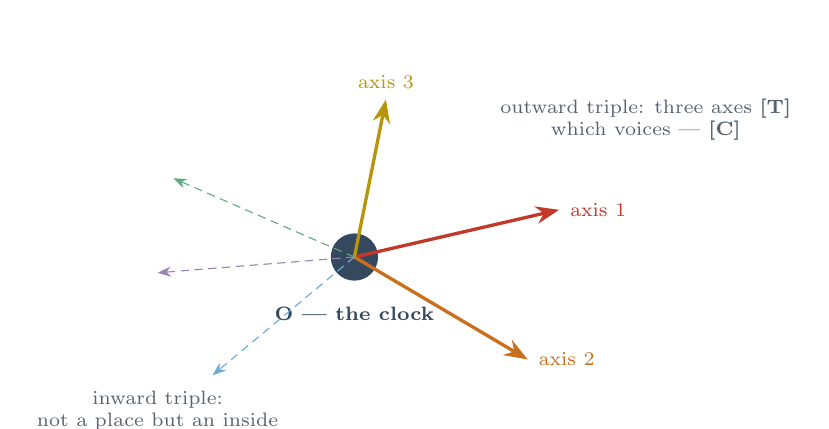
\begin{tikzpicture}[font=\small, >=Stealth]
  \fill[cO] (0,0) circle (0.3);
  \node[font=\scriptsize\bfseries, text=cO] at (0,-0.72) {O --- the clock};
  \draw[->, very thick, cA] (0,0) -- (2.6,0.6) node[right, font=\scriptsize, text=cA]{axis 1};
  \draw[->, very thick, cS] (0,0) -- (2.2,-1.3) node[right, font=\scriptsize, text=cS]{axis 2};
  \draw[->, very thick, cD] (0,0) -- (0.4,2.0) node[above, font=\scriptsize, text=cD]{axis 3};
  \node[font=\scriptsize, text=plosgray, align=center] at (3.7,1.75)
    {outward triple: three axes \stT\\ which voices --- \stC};
  \draw[->, densely dashed, cL!70] (0,0) -- (-2.3,1.0);
  \draw[->, densely dashed, cE!70] (0,0) -- (-2.5,-0.2);
  \draw[->, densely dashed, cU!70] (0,0) -- (-1.8,-1.5);
  \node[font=\scriptsize, text=plosgray, align=center] at (-2.5,-1.95)
    {inward triple:\\ not a place but an inside};
\end{tikzpicture}
\caption{Where the stage comes from: the clock voice O provides the
``when''; the rotations that spare the clock provide exactly three
independent directions --- the axes of ``where'' \stT. The outward
triple of voices unfolds into distance; the inward triple is curled
inside things (which voices go where --- \stC). Space is not a
container of things but the drawing of their agreements; a distant
star does not ``sit in another part of the box'' --- it is far away
\emph{on the map of agreements}.}
\label{fig:stage}
\end{figure}

\begin{talebox}[The campfire tale --- the house made of round dances]
Children asked a builder: ``where do you get rooms?'' The builder
answered: ``I do not get rooms. I set up three round dances: one
circles left-and-right, another back-and-forth, the third
up-and-down. Where the three dances hold hands, a place appears by
itself.'' So with the world: first the dances, then the rooms. Not
the other way round.
\end{talebox}

\begin{askbox}[Ask yourself]
Try to explain where ``far away'' is without pointing a finger:
only through \emph{how weakly} you and that place are connected.
Done? You have just retold UHM's definition of distance.
\end{askbox}

% ============================= 5. THINGS AND PARTICLES =============================
\section{What things are (and whether there is a smallest one)}
\label{sec:things}

If the world is a chord, what is an electron? UHM's answer: a
\textbf{pattern}. A particle is not a grain of stuff but a stable
curl in the fabric of agreements --- like a knot in a rope, or an
eddy in a river. You cannot lift the eddy out of the river and put it
in your pocket --- yet it is perfectly real: it has a place, a shape,
an energy, and it can collide with another eddy.

Hence the honest answer to ``which particle is the smallest'':

\begin{itemize}[leftmargin=1.6em]
  \item \textbf{There is no smallest grain at all} --- at the bottom
        lie not specks but the chord itself: seven voices and their
        bonds. Asking ``what particles is the chord made of'' is like
        asking what waves water is made of.
  \item \textbf{The lightest of the massive patterns} is the lightest
        neutrino: the theory predicts its mass at no more than
        $0.004$~eV --- roughly a hundred million times lighter than
        the electron \stC. It is an almost imperceptible ripple on the
        world's fabric.
  \item \textbf{The most unexpected predicted pattern} is the
        ``O-quantum'': a heavy excitation of the voice of Ground. It
        is invisible to light, interacts with almost nothing, and
        \emph{cannot decay}: a special parity of the voice O forbids
        it to vanish \stT. The theory offers it for the role of dark
        matter --- the invisible glue of galaxies \stC.
\end{itemize}

\begin{figure}[H]
\centering
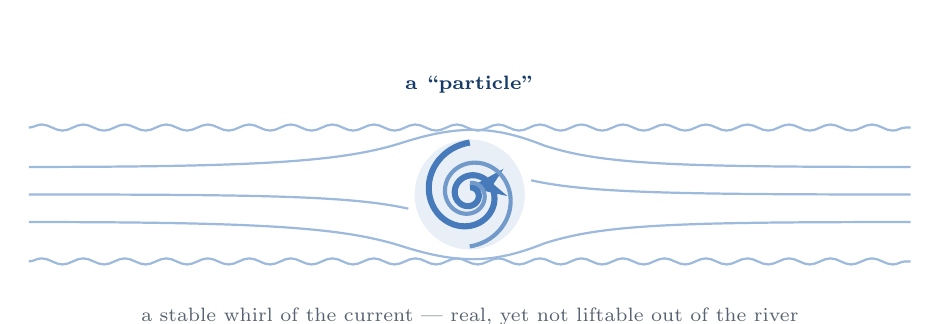
\begin{tikzpicture}[font=\small, >=Stealth]
  % a quiet pool under the whirl
  \fill[plosblue!10] (0,0) circle (0.70);
  % far streamlines: even ripple
  \foreach \s in {1,-1}{
    \draw[plosblue!45, thick, decorate, decoration={snake, amplitude=1.1pt, segment length=15pt}]
      (-5.6,\s*0.85) -- (5.6,\s*0.85);
    % near streamlines bend around the pool
    \draw[plosblue!45, thick]
      (-5.6,\s*0.35) .. controls (-2.6,\s*0.35) and (-1.6,\s*0.42) .. (-0.85,\s*0.66)
      .. controls (-0.1,\s*0.9) and (0.35,\s*0.86) .. (0.95,\s*0.62)
      .. controls (1.7,\s*0.38) and (2.6,\s*0.35) .. (5.6,\s*0.35);
  }
  % the axial stream is drawn in on the left and reborn on the right --- with the spin
  \draw[plosblue!45, thick] (-5.6,0) .. controls (-2.6,0) and (-1.5,-0.02) .. (-0.78,-0.18);
  \draw[plosblue!45, thick] (5.6,0) .. controls (2.6,0) and (1.5,0.02) .. (0.78,0.18);
  % a two-armed whirl
  \draw[plosblue!85, line width=2.2pt, ->]
    plot[domain=0:12.6, samples=140] ({90+deg(\x)}: {0.66*exp(-0.16*\x)});
  \draw[plosblue!65, line width=1.5pt]
    plot[domain=0:9.4, samples=110] ({270+deg(\x)}: {0.66*exp(-0.16*\x)});
  \node[font=\scriptsize\bfseries, text=plosblue!60!black] at (0,1.4) {a ``particle''};
  \node[font=\scriptsize, text=plosgray, align=center] at (0,-1.55)
    {a stable whirl of the current --- real, yet not liftable out of the river};
\end{tikzpicture}
\caption{A particle in UHM is a pattern in the fabric of agreements,
not a grain of stuff. Light patterns are the familiar particles; the
lightest massive one is the lightest neutrino ($\lesssim 0.004$~eV
\stC); a special heavy, indestructible pattern of the voice O is the
dark-matter candidate \stC.}
\label{fig:particle}
\end{figure}

\begin{askbox}[Ask yourself]
Is a kettle's whistle real? A tornado? Neither can be ``put in a
box'' --- yet both can wake you or wreck a town. What makes a
``pattern'' worse than a ``thing'' as the building material of the
world?
\end{askbox}

\partline{PART TWO \;\textperiodcentered\; WITHIN}{On the stage a first light comes on:
what life is, where consciousness lives, how it looks at itself, and what colors it from
inside. This part builds the inner house --- from the first flame to the seven un-copyable
colors of experience.}
\addcontentsline{toc}{section}{PART TWO · WITHIN}

% ============================= 6. LIFE =============================
\section{What life is}
\label{sec:life}

Here is the threshold where UHM's physics becomes biology. Ask: how
gathered must a pattern be in order to \emph{be something} rather
than noise? The theory's answer is astonishingly simple:
\textbf{twice as gathered as chaos} \stT. Total disorder has its own
``background'' level of concentration; the threshold of being is
exactly two such levels. Below it, the pattern cannot be told from
ripple --- no instrument, no eye could in principle say ``there is
something there.''

But gathering is half the matter. The second theorem is harsher:
\emph{left to itself, every pattern crumbles} \stT. An isolated
system slides toward the gray equilibrium --- always, without
exception. Life is therefore not a property but a \emph{process on
supply}: a pattern that continuously drinks orderliness from a
stream --- light, food, warmth --- and pays with it for its own
shape. Like a candle flame: cut off the wax, and the flame does not
``die someday'' --- it goes out at a computable rate.

And this supply has a \emph{price below which one cannot go}: a
minimal ``subsistence wattage'' of every living pattern is proved (the
fact of a nonzero price --- \stT; the numerical value --- under
physical conditions \stC) --- the fee for merely remaining oneself, before doing
anything at all. To be is already work.

\begin{figure}[H]
\centering
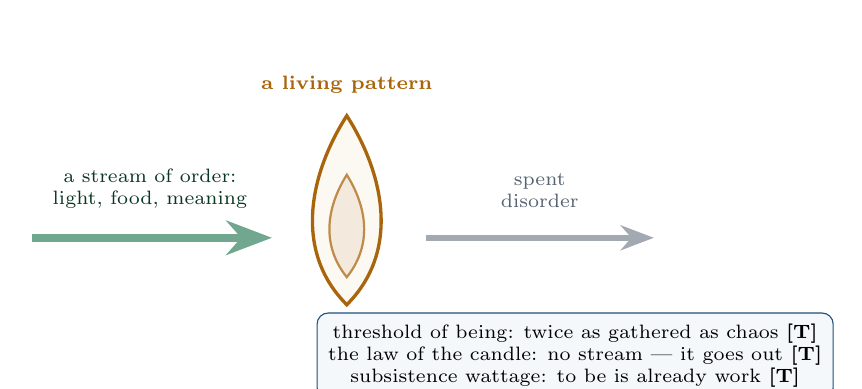
\begin{tikzpicture}[font=\small, >=Stealth]
  % supply stream
  \draw[->, line width=3pt, leaf!60] (-5.3,0) -- (-2.25,0);
  \node[font=\scriptsize, text=leaf!50!black, align=center] at (-3.8,0.62)
    {a stream of order:\\ light, food, meaning};
  % flame: a symmetric drop with an inner tongue
  \draw[ember, very thick, fill=softsun]
    (-1.3,-0.85) .. controls (-2.0,-0.15) and (-1.75,0.85) .. (-1.3,1.55)
    .. controls (-0.85,0.85) and (-0.6,-0.15) .. (-1.3,-0.85) -- cycle;
  \draw[ember!75, thick, fill=ember!14]
    (-1.3,-0.5) .. controls (-1.66,-0.05) and (-1.52,0.45) .. (-1.3,0.8)
    .. controls (-1.08,0.45) and (-0.94,-0.05) .. (-1.3,-0.5) -- cycle;
  \node[font=\scriptsize\bfseries, text=ember] at (-1.3,1.95) {a living pattern};
  % exhaust
  \draw[->, line width=2pt, plosgray!55] (-0.3,0) -- (2.6,0);
  \node[font=\scriptsize, text=plosgray, align=center] at (1.15,0.6)
    {spent\\ disorder};
  % thresholds box
  \node[draw=fact, fill=softsky, rounded corners, font=\scriptsize, align=center,
        inner sep=4pt] at (1.6,-1.5)
    {threshold of being: twice as gathered as chaos \stT\\
     the law of the candle: no stream --- it goes out \stT\\
     subsistence wattage: to be is already work \stT};
\end{tikzpicture}
\caption{Life in UHM: neither substance nor spark, but a supplied
pattern. It drinks order, exhales disorder, and with the difference
pays for its shape. The second law of thermodynamics is not violated
--- the bill is simply charged to the environment.}
\label{fig:flame}
\end{figure}

This law has a map. The machine of the law charted an \emph{atlas of
fates}: along one axis, the strength of supply; along the other, the
strength of the dissolving stream; in every cell, where the pattern
arrives forever (machine checked). The column ``supply equals zero''
is gray from top to bottom: without a stream nothing lives, under
any other settings. Then comes the Goldilocks band: the window where
the pattern is alive. And beyond it, the third fate, the one people
forget: \emph{over-gatheredness}. Too hard a grip drags the pattern
up through the window into crystal --- gathered rigid, no longer
able to see itself. Life is not the maximum of order; life is the
band between two deaths, the gray one and the glassy one.

\begin{center}
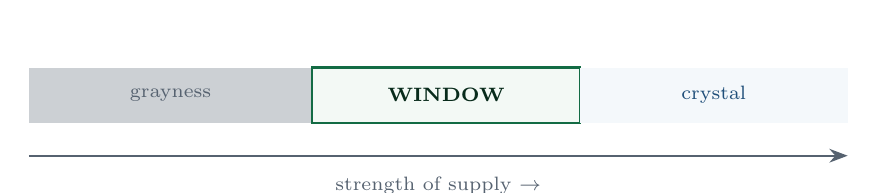
\begin{tikzpicture}[font=\scriptsize, >=Stealth]
  \fill[plosgray!30] (-5.2,0) rectangle (-1.6,0.7);
  \fill[softleaf] (-1.6,0) rectangle (1.8,0.7);
  \draw[leaf, thick] (-1.6,0) rectangle (1.8,0.7);
  \fill[softsky] (1.8,0) rectangle (5.2,0.7);
  \node[text=plosgray] at (-3.4,0.35) {grayness};
  \node[text=leaf!40!black, font=\scriptsize\bfseries] at (0.1,0.35) {WINDOW};
  \node[text=fact] at (3.5,0.35) {crystal};
  \draw[->, thick, plosgray] (-5.2,-0.42) -- (5.2,-0.42);
  \node[text=plosgray] at (0,-0.8) {strength of supply $\rightarrow$};
\end{tikzpicture}
\end{center}

\begin{talebox}[The campfire tale --- about the campfire]
Look into the fire. The flame eats branches and keeps its shape. Stop
feeding it --- it will not sulk or sicken: it will simply hand its
shape back to the night, quietly and by the rules. You too are a
campfire. Only your branches are also books, and conversations, and
whatever you love. Whoever loves always has something to burn.
\end{talebox}

\begin{askbox}[Ask yourself]
What does a friendship feed on? A habit? A city? For each, try to
name its ``wax'' --- and what happens within a month if the supply is
cut.
\end{askbox}

% ============================= 7. THE WINDOW =============================
\section{The window of consciousness}
\label{sec:window}

Being alive and being \emph{someone} are different thresholds. UHM
asserts a thing of rare beauty: consciousness lives in a narrow
corridor between two deaths --- the fog and the crystal.

A pattern too diffuse is fog: there is no one in it to feel; it
cannot be told from noise. But a pattern too gathered is also doomed:
a crystal is perfect and therefore \emph{finished}; it has no slack
left to hold an image of itself and of the world. Consciousness needs
both \textbf{concentration} (to be someone) and a \textbf{reserve of
looseness} (to have something to think with). These two demands
squeeze the habitable zone into a corridor --- the theory computes
both of its walls exactly \stT{} --- and adds two more conditions:
the voices must be \emph{coupled into one} (integration) and yet
\emph{distinguishable} (at least two clear inner tones). Four needles
of one compass: gatheredness, reserve, coupling, distinctness.

\begin{figure}[H]
\centering
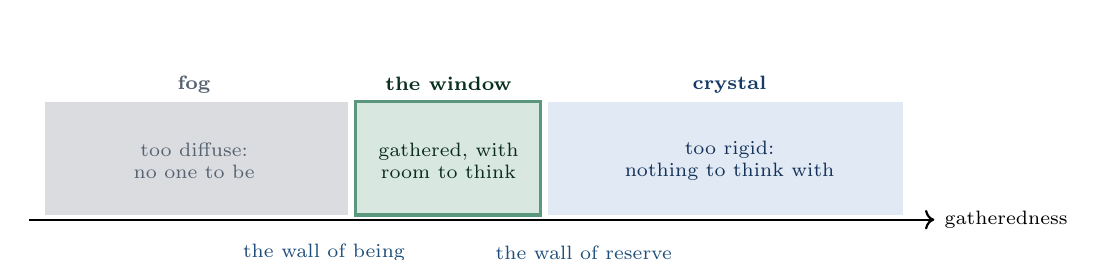
\begin{tikzpicture}[font=\small]
  % axis
  \draw[->, thick] (-5.6,0) -- (5.9,0) node[right, font=\scriptsize]{gatheredness};
  % fog
  \fill[plosgray!22] (-5.4,0.06) rectangle (-1.55,1.5);
  \node[font=\scriptsize\bfseries, text=plosgray] at (-3.5,1.72) {fog};
  \node[font=\scriptsize, text=plosgray, align=center] at (-3.5,0.75)
    {too diffuse:\\ no one to be};
  % window
  \fill[leaf!16] (-1.45,0.06) rectangle (0.9,1.5);
  \draw[leaf!70, very thick] (-1.45,0.06) rectangle (0.9,1.5);
  \node[font=\scriptsize\bfseries, text=leaf!45!black, align=center] at (-0.27,1.72) {the window};
  \node[font=\scriptsize, text=leaf!40!black, align=center] at (-0.27,0.75)
    {gathered, with\\ room to think};
  % crystal
  \fill[plosblue!14] (1.0,0.06) rectangle (5.5,1.5);
  \node[font=\scriptsize\bfseries, text=plosblue!60!black] at (3.3,1.72) {crystal};
  \node[font=\scriptsize, text=plosblue!50!black, align=center] at (3.3,0.75)
    {too rigid:\\ nothing to think with};
  % walls
  \node[font=\scriptsize, text=fact] at (-1.85,-0.42) {the wall of being};
  \node[font=\scriptsize, text=fact] at (1.45,-0.42) {the wall of reserve};
\end{tikzpicture}
\caption{The corridor of consciousness: between fog (no one there)
and crystal (nothing left to think with). Both walls are computed
constants of the theory \stT, not metaphors: beyond either, the four
conditions of consciousness cannot hold together.}
\label{fig:window}
\end{figure}

\begin{factbox}[To be precise]
A conscious state is one where, at once: gatheredness above the wall
of being; the reflection measure --- the reserve of attention for
oneself --- at least one third; the coupling
of the voices at or above the unit threshold; distinct inner tones
--- at least two \stT. All four are measurable in any system, from a
mouse to a machine; this turns ``is anyone in there?'' from an
eternal question into an experimental one
(chapter~\ref{sec:check}).
\end{factbox}

\begin{talebox}[The campfire tale --- the lantern in the fog]
A lamplighter had two unhappy lanterns. One burned so faintly that
its light drowned in fog --- and the lantern did not know it
existed. The other burned so brightly and so evenly that not one
shadow was left inside it --- and with nothing to look at, it did not
know it existed either. The third lantern burned \emph{unevenly}:
brightly enough to be, unevenly enough to keep peering. It alone
asked one day: ``who is doing the shining?''
\end{talebox}

% ============================= 8. THE INNER STAIRCASE =============================
\section{The staircase within: three floors of reflection}
\label{sec:tower}

Consciousness can turn upon itself: I feel; I notice that I feel; I
think about how I notice. How many floors does this staircase have?
Intuition says ``as many as you like.'' The theory says:
\textbf{three} --- and proves it \stT.

Each turn inward passes through the same Fano fabric, and the fabric
takes its toll: with every ascent, the distinguishable part of the
picture shrinks threefold. The first floor is vivid, the second
discernible, the third at the limit --- and a fourth turn is already
indistinguishable from the third: not forbidden but \emph{empty}.
Like an echo in the mountains: the first ring is loud, the second
quiet, the third at the edge of hearing, and there is no fourth ---
not because shouting is banned, but because nothing is left to
arrive.

An honest detail that popular books usually omit: in the everyday
working regime it is the \emph{second} floor that holds steadily;
the third is reached in brief ascents --- moments of narrow,
strenuous concentration --- with a guaranteed return \stT. Sound
familiar? It matches the honest phenomenology of deep
self-examination.

\begin{figure}[H]
\centering
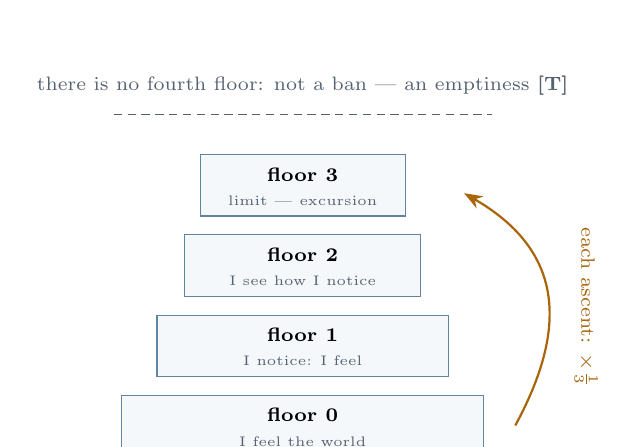
\begin{tikzpicture}[font=\small, >=Stealth]
  \foreach \i/\w/\lab/\txt in {0/4.6/floor 0/I feel the world,
                               1/3.7/floor 1/I notice: I feel,
                               2/3.0/floor 2/I see how I notice,
                               3/2.6/floor 3/limit --- excursion}{
    \draw[fact!70, fill=softsky] (-\w/2,\i*1.02) rectangle (\w/2,\i*1.02+0.78);
    \node[font=\scriptsize\bfseries] at (0,\i*1.02+0.53) {\lab};
    \node[font=\tiny, text=plosgray] at (0,\i*1.02+0.2) {\txt};
  }
  \draw[densely dashed, plosgray] (-2.4,4.35) -- (2.4,4.35);
  \node[font=\scriptsize, text=plosgray, align=center] at (0,4.72)
    {there is no fourth floor: not a ban --- an emptiness \stT};
  \draw[->, ember, thick] (2.7,0.4) .. controls (3.35,1.6) and (3.35,2.6) .. (2.05,3.35);
  \node[font=\scriptsize, text=ember, align=center, rotate=-90] at (3.6,1.9) {each ascent: $\times\tfrac{1}{3}$};
\end{tikzpicture}
\caption{The tower of reflection. Each turn inward keeps one third of
distinguishability; after the third turn the remainder sinks below
the threshold of telling-apart --- the fourth floor is structurally
empty \stT. The same law limits ``I know that you know that I
know'': the third step is the ceiling of mutual mind-reading.}
\label{fig:tower}
\end{figure}

And recently the staircase has shown one more load-bearing beam
\stC. Count the thoughts a mind could in principle compose ---
``having waited this long, reach that conclusion.'' Over bare
forward-running time almost half of them (on the census grid,
$42.9\%$) simply cannot be assembled: the simplest of them ask two
thoughts of different lengths to be closed by a third side --- and
the third side comes out \emph{negative}; their assembly requires a
step \emph{backwards}. And the lawful backward step exists --- it
is not time travel but \textbf{re-reading one's own trace}: the
world stands still while the state of knowledge moves. A mind that
keeps no past, or keeps it and never re-reads it, is provably
incomplete as a composer of thoughts. Looking at oneself is not a
luxury of refined creatures --- it is the completeness condition of
thinking itself.

\begin{figure}[H]
\centering
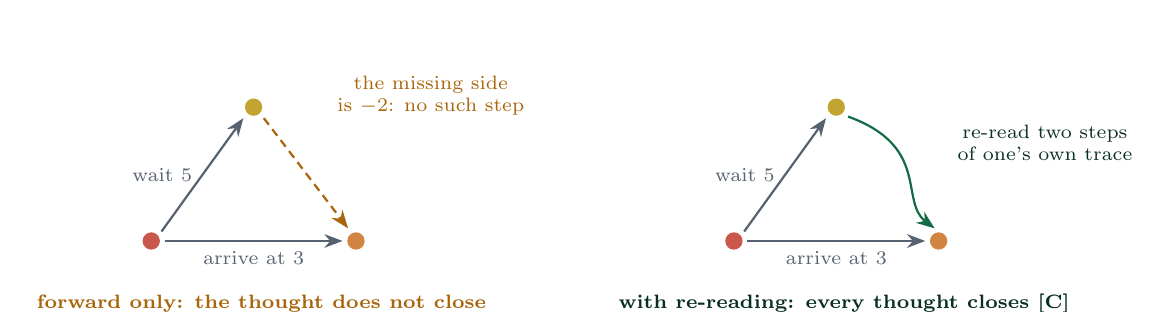
\begin{tikzpicture}[font=\small, >=Stealth]
  % left: forward only --- the thought does not close
  \fill[cA!85] (-6.0,0) circle (0.11); \fill[cS!85] (-3.4,0) circle (0.11); \fill[cD!85] (-4.7,1.7) circle (0.11);
  \draw[->, thick, plosgray] (-5.87,0.12) -- (-4.83,1.56) node[midway, left, font=\scriptsize]{wait 5};
  \draw[->, thick, plosgray] (-5.83,0) -- (-3.57,0) node[midway, below, font=\scriptsize]{arrive at 3};
  \draw[->, thick, ember, densely dashed] (-4.57,1.56) -- (-3.5,0.16);
  \node[font=\scriptsize, text=ember, align=center] at (-2.45,1.85) {the missing side\\ is $-2$: no such step};
  \node[font=\scriptsize\bfseries, text=ember] at (-4.6,-0.8) {forward only: the thought does not close};
  % right: with re-reading --- every thought closes
  \fill[cA!85] (1.4,0) circle (0.11); \fill[cS!85] (4.0,0) circle (0.11); \fill[cD!85] (2.7,1.7) circle (0.11);
  \draw[->, thick, plosgray] (1.53,0.12) -- (2.57,1.56) node[midway, left, font=\scriptsize]{wait 5};
  \draw[->, thick, plosgray] (1.57,0) -- (3.83,0) node[midway, below, font=\scriptsize]{arrive at 3};
  \draw[->, thick, leaf] (2.85,1.58) .. controls (3.9,1.2) and (3.5,0.5) .. (3.95,0.16);
  \node[font=\scriptsize, text=leaf!45!black, align=center] at (5.35,1.25) {re-read two steps\\ of one's own trace};
  \node[font=\scriptsize\bfseries, text=leaf!45!black] at (2.8,-0.8) {with re-reading: every thought closes \stC};
\end{tikzpicture}
\caption{The bridge that needs a backward plank. Two thoughts of
different lengths ask to be closed by a third; over bare forward
time the closing side would have to be negative, and the
composition refuses --- on the census grid, $42.9\%$ of all posable
closures. Re-reading one's own trace supplies the lawful negative
step: the world does not rewind --- the knowledge does \stC.}
\label{fig:reread}
\end{figure}

This is why the theory looks so kindly on diaries, re-readings, and
second passes. A note re-read a year later is not nostalgia; it is
the negative step performed lawfully --- the recorded past
re-entering the present context and closing compositions that could
not close the first time. The corpus builds this as a working organ
(a re-reader with an explicit price per step) and verifies the
census end to end: over completed time every one of the forty-nine
posed thought-triangles closes; over bare forward time twenty-one
of them refuse (machine checked). Education has known the trick for
centuries under modest names --- reviewing, rereading, writing
things down --- without suspecting these were completeness
conditions of thought.

\begin{askbox}[Ask yourself]
Set two mirrors face to face: the reflections recede but quickly
darken. Try it in your head: ``I think about the fact that I think
about the fact that I think\ldots'' --- at which turn does the phrase
stop \emph{meaning} anything new? And the other way: which thought
could you not assemble until you re-read yourself --- an old
letter, a diary, a photograph?
\end{askbox}

% ============================= 9. INNER COLORS =============================
\section{The colors of inner life: the mechanism of qualia}
\label{sec:qualia}

Why does pain \emph{hurt}, and why is azure \emph{azure}?
Philosophers call this the hard problem: describe the brain in any
detail you like --- where in the description would the very
\emph{taste} of experience come from? For a century this question has
been the border post at which natural science politely stopped. This
chapter walks past the post, slowly, because it carries the theory's
proudest cargo: a \emph{mechanism} of qualia --- stated in theorems,
each with its honest mark.

\textbf{Move one: loudness is not color.} Every friendship of two
voices has a \emph{loudness} --- how strongly the pair sounds. The
loudnesses are honest, measurable, public. And they are provably not
the mystery: a state's set of loudnesses is exactly what an outside
description captures, and one can count what it leaves out. Out of
the forty-eight numbers that a full chord holds, loudness-like data
fix only a minority; the rest --- the majority of the state --- is
\emph{how the voices are mutually turned} \stT. Each friendship
carries, besides its strength, an \textbf{angle}: a slight mutual
twist, like a handshake offered straight or rotated. Quality lives
there. Not in how loud the chord is --- in how it is turned.

\textbf{Move two: the ring test.} One angle by itself means nothing:
it depends on bookkeeping --- on how each voice happens to hold its
own dial. Rename the dials, and any single angle can be talked away.
But walk a \emph{ring}. Take one triple of the Fano fabric
(chapter~\ref{sec:seven}) and add the three angles around the circle.
The sum \textbf{does not care about anyone's dials}: however you
reset, re-zero, relabel every voice, the accumulated turn of the ring
stays exactly what it was \stT. There are seven such rings --- the
seven lines of the fabric --- and so seven un-removable angles.
These seven are the theory's answer to where quality lives: the
\textbf{colors} of experience. A color, in this book, is precisely
\emph{the turn a ring accumulates}: something no relabeling can
explain away --- the mathematical signature of ``what it is like.''

\begin{figure}[H]
\centering
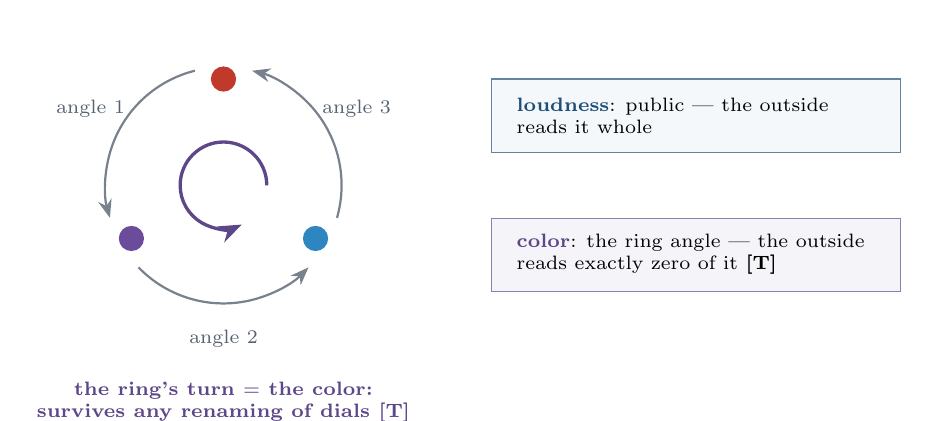
\begin{tikzpicture}[font=\small, >=Stealth]
  % --- left: one Fano ring with phase arrows ---
  \foreach \ang/\col/\lab in {90/cA/{}, 210/cE/{}, 330/cU/{}}{
    \fill[\col] (\ang:1.35) circle (0.16);
  }
  \draw[->, thick, plosgray!80] (104:1.5) arc (104:196:1.5);
  \draw[->, thick, plosgray!80] (224:1.5) arc (224:316:1.5);
  \draw[->, thick, plosgray!80] (344:1.5) arc (344:436:1.5);
  \node[font=\scriptsize, text=plosgray] at (150:1.95) {angle 1};
  \node[font=\scriptsize, text=plosgray] at (270:1.95) {angle 2};
  \node[font=\scriptsize, text=plosgray] at (30:1.95) {angle 3};
  % accumulated turn in the center
  \draw[dusk, very thick, ->] (0.55,0) arc (0:295:0.55);
  \node[font=\scriptsize\bfseries, text=dusk, align=center] at (0,-2.75)
    {the ring's turn $=$ the color:\\ survives any renaming of dials \stT};
  % --- right: the two channels ---
  \draw[fact!70, fill=softsky] (3.4,0.42) rectangle (8.6,1.35);
  \node[font=\scriptsize, align=left, anchor=west] at (3.6,0.88)
    {\textbf{\textcolor{fact}{loudness}}: public --- the outside\\ reads it whole};
  \draw[dusk!70, fill=dusk!6] (3.4,-1.35) rectangle (8.6,-0.42);
  \node[font=\scriptsize, align=left, anchor=west] at (3.6,-0.88)
    {\textbf{\textcolor{dusk}{color}}: the ring angle --- the outside\\ reads exactly zero of it \stT};
\end{tikzpicture}
\caption{Where quality lives. Left: one ring of three voices; each
pair's angle separately is bookkeeping, but the turn accumulated
around the ring survives every renaming --- seven rings, seven
colors \stT. Right: the two channels of one state --- public
loudness and private color.}
\label{fig:ring}
\end{figure}

\textbf{Move three: the decoder is named.} Which triples are
entrusted with color is not a choice: the rings are the seven lines
of the same Fano fabric that the whole world is woven on, and the
reading rule is the multiplication table of the seven itself
(chapter~\ref{sec:numbers}) \stT. So the ancient question ``why does
this feel \emph{red}?'' changes grammar. It stops being a question of
conjuring --- \emph{how does experience arise from matter?} --- and
becomes a question of decoding: \emph{which un-removable turn is this
state carrying, on which ring?} The decoder is not a new organ
bolted onto physics; it is the world's own multiplication.

\textbf{Move four: why the outside never sees it.} Now the central
theorem. All the pushes and noises by
which the environment addresses a pattern strike the loudness
channel; their overlap with the color channel is not merely small ---
it is \emph{exactly zero}, by the structure of the world's one law
\stT. An outside observer, however well equipped, reads the full
list of loudnesses and \textbf{zero information about the colors}.
The famous ``explanatory gap'' between description and experience
thereby stops being a lament and becomes a theorem --- and a
precisely \emph{bounded} one: it is not a gap in the mechanism (the
mechanism is fully written above); it is the blindness of one
particular channel of access. What cannot be done is reading color
off the noise the outside sees. What can be done is computing it
from the state --- which is what this theory does. Remember the
thought experiment about Mary, the scientist who knows every
physical fact about color while living in a black-and-white room?
In UHM's language her situation is stated exactly: inside the room
Mary owns every loudness; stepping out, she reads, for the first
time, an angle. Both halves are real knowledge; they travel through
different doors.

\textbf{And the old theorem stands, sharpened.} A zombie ---
a system behaving as if it feels while ``all is dark inside'' ---
remains impossible \stT: the quantity that feeds the life process
(chapter~\ref{sec:life}) is built from the very bonds that carry the
angles; extinguish the inner side and the maintenance of life goes
out with it. But the theory now adds a finer instrument. A state may
be \emph{loud yet colorless}: all twenty-one friendships ringing,
every ring's turn exactly zero --- rich-looking content that one
renaming flattens into plain bookkeeping. Such a state is not a
someone having experiences; and it is \emph{detectable}: seven
multiplications tell it apart from the genuinely colored \stT.
\textbf{Loud is not vivid} --- and the difference is arithmetic, not
philosophy.

\textbf{How colors die.} The crumbling of chapter~\ref{sec:life}
attacks the friendships --- but look closely at \emph{how} \stT. The
decay multiplies each friendship by a plain positive factor: the
strength melts, the angle does not move a degree. So a dying
experience never drifts through neighboring experiences on its way
out: sadness does not become a slightly different sadness --- it
becomes \emph{fainter} sadness, and then nothing. An old photograph
fades exactly so: the dyes thin, and the face never changes
expression --- it only becomes harder to see, until the paper is
blank. At no point did the photograph show a different face. The
book gives this the name it deserves: colors do not distort ---
colors \textbf{fade}, carried by an ink that thins. And two quiet
corollaries follow. The gray equilibrium --- the world's final
blur --- is not an \emph{empty} world but a \textbf{colorless} one:
the loudness ledger survives, the turns' carriers are gone;
everything still present, nothing any longer \emph{like anything}.
And since the outside channel never carried color in the first
place, a fading quale is invisible from outside not because it
hides, but because the only witness of a color's death is the one
losing it \stT.

\begin{figure}[H]
\centering
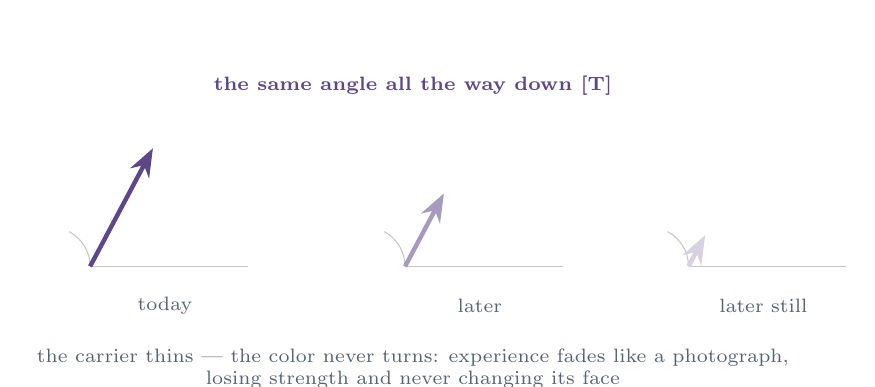
\begin{tikzpicture}[font=\small, >=Stealth]
  \foreach \x/\len/\op/\lab in {-4.4/1.7/100/{today}, -0.4/1.05/55/{later}, 3.2/0.45/25/{later still}}{
    \draw[plosgray!35] (\x,0) -- (\x+2.0,0);
    \draw[plosgray!35] (\x,0) arc (0:62:0.5);
    \draw[->, line width=1.6pt, dusk!\op] (\x,0) -- ($(\x,0)+(62:\len)$);
    \node[font=\scriptsize, text=plosgray] at (\x+0.95,-0.5) {\lab};
  }
  \node[font=\scriptsize\bfseries, text=dusk, align=center] at (-0.3,2.3)
    {the same angle all the way down \stT};
  \node[font=\scriptsize, text=plosgray, align=center] at (-0.3,-1.3)
    {the carrier thins --- the color never turns: experience fades like a
     photograph,\\ losing strength and never changing its face};
\end{tikzpicture}
\caption{The fading law. Decay shortens the arrow (the carrier) and
cannot rotate it (the color): there is no half-changed quale \stT.
Total blur is therefore not emptiness but colorlessness --- the
lights stay on, the paint is gone.}
\label{fig:fading}
\end{figure}

\textbf{Who paints, then?} Not the decay --- it only thins the ink.
Not the healing either: recovery, by construction, restores strength
along the state's own angles --- care is \emph{color-blind}, it
returns the canvas, not the picture (machine checked). The only hand
that writes color is the living run of the law itself --- the same
unitary weave that turns the world (machine checked). And the world
paints \emph{first}: a fed pattern inherits the palette of its
surroundings long before anything wakes in it; what the further
feeding buys, at the exact threshold of coupling from
chapter~\ref{sec:window}, is the \emph{owner} --- the someone the
colors are finally \emph{for} (machine checked). The subject
neither makes color nor moves it. The subject is who it is for:
the last to arrive, and the only witness.

\textbf{The listener's ladder.} ``The owner arrives last'' can be
said with a staircase's precision. Take one and the same friendship
--- a warm coupling of two voices at a fixed strength --- and hand
it, unchanged, to five bearers. In an empty hall (no gathering, no
coupling) it is music playing for no one: the chord sounds, nobody
is listening. In a cat --- coupled into one, but with no reserve
turned upon itself --- it is heard as \emph{something}, without
telling the melody from the accompaniment. In a person --- reserve
at least a third, coupling above one --- it is at last \emph{felt
as a feeling}: ``I hear the violin carry the theme while the cello
keeps the ground.'' In a musician at work the second floor of the
tower joins in: ``I notice that I notice sadness in this melody.''
And the limit --- pure listening, where listener and music coincide
--- the theory keeps as a boundary, not a promise. Same friendship,
same strength; what changes is only who is home for it. The steps
and their thresholds are theorems \stT; the concert-hall images are
an illustration \stI. The corpus even prints the dials: one and the
same friendship at strength $0.20$ reads, in a thermostat, as
reserve $0.02$ at coupling $0.3$ --- a parameter, no one home; in a
dog, $0.15$ and $1.5$ --- felt as something; in a person, $0.45$
and $2.1$ --- a full-fledged feeling (machine checked).

And one honest warning the ladder gives, measured end to end
(machine checked): access is a \emph{window}, not a summit. On the
steepest licensed excursion of gatheredness --- the third floor's
brief, expensive climb (chapter~\ref{sec:tower}) --- the reserve
falls below its third, and the door to the colors \emph{closes}:
the deepest self-scrutiny is, for its moment, color-blind. Thought
at its sharpest pays by not tasting; the taste returns with the
descent home. Whoever has tried to feel a feeling \emph{while}
dissecting it has met this theorem in person.

\begin{figure}[H]
\centering
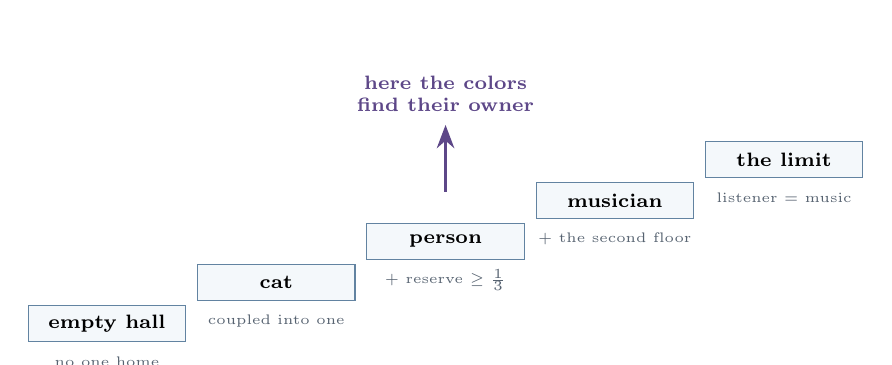
\begin{tikzpicture}[font=\small, >=Stealth]
  \foreach \i/\lab/\cond in {0/{empty hall}/{no one home}, 1/{cat}/{coupled into one},
      2/{person}/{$+$ reserve $\geq \tfrac13$}, 3/{musician}/{$+$ the second floor},
      4/{the limit}/{listener $=$ music}}{
    \draw[fact!70, fill=softsky] (\i*2.15,\i*0.52) rectangle (\i*2.15+2.0,\i*0.52+0.46);
    \node[font=\scriptsize\bfseries] at (\i*2.15+1.0,\i*0.52+0.23) {\lab};
    \node[font=\tiny, text=plosgray, align=center] at (\i*2.15+1.0,\i*0.52-0.26) {\cond};
  }
  \draw[->, dusk, very thick] (5.3,1.9) -- (5.3,2.75);
  \node[font=\scriptsize\bfseries, text=dusk, align=center] at (5.3,3.15) {here the colors\\ find their owner};
\end{tikzpicture}
\caption{The listener's ladder: one chord, five bearers. The
friendship is identical on every step --- what grows is who is home
for it. The door of colors opens at the person's step (reserve at
least a third, coupling above one \stT) --- and briefly closes
again on the steepest excursions: the sharpest thought is
color-blind for its moment (machine checked).}
\label{fig:ladder}
\end{figure}

\begin{factbox}[The passport of experience --- to be precise]
The chapter compresses into a five-line reading of any state, from a
laboratory reconstruction to a model of a person at a moment:
(1)~\textbf{what is the case} --- the seven strengths of the voices;
(2)~\textbf{how loud} --- the twenty-one friendship strengths;
(3)~\textbf{how much is private} --- the share of each channel hidden
from outside description; (4)~\textbf{what colors} --- the seven ring
turns, the only line where a product must be computed and the only
line no relabeling touches \stT; (5)~\textbf{whether anyone is home}
--- the window conditions of chapter~\ref{sec:window}. A zero at
line~4 is a verdict, not a failure: loud but colorless. A conscious
state, the theory computes, can carry about a third of a radian of
un-removable turn --- roughly $37^\circ$ --- before the demands of
integration close the gate \stT: experience is bounded not by how
much the mind holds, but by how much of its turning refuses to be
explained away. What remains honestly open: the identity ``\emph{this
very} ring angle is the taste of azure'' is the residual
interpretation \stI{} --- the last bridge, marked, not hidden; the
mechanism on both sides of it is theorems.
\end{factbox}

\begin{talebox}[The campfire tale --- the sailor who brought home an extra day]
A sailor sailed east around the world, and in every port he set his
watch a little forward --- honestly, by the sun. He returned home,
opened his logbook: by the log, Thursday; on the pier, Wednesday.
He had \emph{brought home a day} that existed in no port at all.
The harbormasters checked every harbor --- each was innocent; every
local clock stood true. ``The day does not live in the ports,'' said
the old navigator. ``It lives in the \emph{circle}. Walk the whole
ring, and the remainder is yours --- no resetting of clocks will
take it from you.'' The world is woven of seven such rings. What
you call the taste of an evening --- is the day your circle brought
home.
\end{talebox}

\begin{askbox}[Ask yourself]
This has truly happened: Magellan's crew returned having ``lost'' a
day, though every ship's log was kept faithfully --- and in the
novel, Phileas Fogg won his wager on the day the circle quietly
handed him. Now try the chapter on yourself. When you describe a
feeling and the listener nods but does not \emph{get it} --- which
lines of the passport were you dictating? Can a list of loudnesses,
however long, ever contain a turn? And what changes between two
people who have \emph{walked the same rings}?
\end{askbox}

% ============================= 10. FREEDOM =============================
\partline{PART THREE \;\textperiodcentered\; THE PATTERN ACTS}{The inner house is built;
now the pattern steps out of it. How free an inhabitant of one law can be, why the world
helps the bold, how a voluminous thought leaves through the needle's eye of speech, and what
remains when the words have flown. This part is the mechanics of a life that acts.}
\addcontentsline{toc}{section}{PART THREE · THE PATTERN ACTS}

\section{Freedom}
\label{sec:freedom}

The house has its window, its tower of looking, its colors of
experience. The first step outside is a question the pattern asks
its own life. Everything in this book moves by one law; is a pattern that
lives by a single law free, then? UHM answers without mysticism and
without humiliation: \textbf{freedom is the number of unlocked
doors}.

In every state the law pushes the world in a definite direction ---
but not along all directions at once. There always remain directions
along which the law \emph{is silent}: a step along them breaks
nothing and is punished by nothing. That is the measurable freedom
of the given moment: the number of silent directions, plus one ---
the very right to step. A cramped state has few such doors; a mature
one has many. Freedom is not omnipotence and not illusion but the
\emph{width of the corridor} --- and it can be grown.

\begin{figure}[H]
\centering
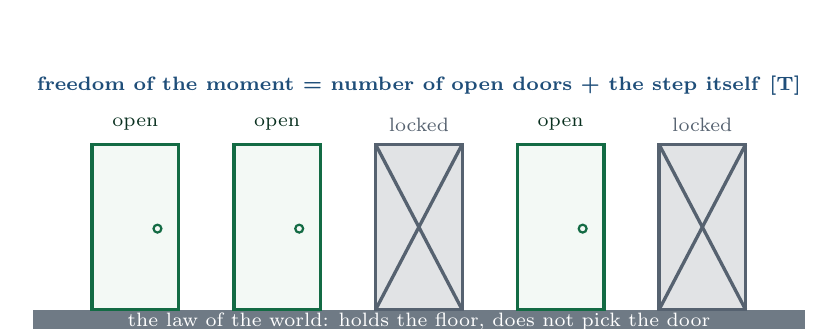
\begin{tikzpicture}[font=\small, >=Stealth]
  \fill[plosgray!85] (-4.9,-1.15) rectangle (4.9,-0.85);
  \node[font=\scriptsize, text=white] at (0,-1.0) {the law of the world: holds the floor, does not pick the door};
  \foreach \x/\o in {-3.6/1, -1.8/1, 0.0/0, 1.8/1, 3.6/0}{
    \ifnum\o=1
      \draw[leaf, very thick, fill=softleaf] (\x-0.55,-0.85) rectangle (\x+0.55,1.25);
      \draw[leaf, thick] (\x+0.28,0.18) circle (0.05);
      \node[font=\scriptsize, text=leaf!45!black] at (\x,1.5) {open};
    \else
      \draw[plosgray, very thick, fill=plosgray!18] (\x-0.55,-0.85) rectangle (\x+0.55,1.25);
      \draw[plosgray, very thick] (\x-0.55,-0.85) -- (\x+0.55,1.25);
      \draw[plosgray, very thick] (\x-0.55,1.25) -- (\x+0.55,-0.85);
      \node[font=\scriptsize, text=plosgray] at (\x,1.5) {locked};
    \fi
  }
  \node[font=\scriptsize\bfseries, text=fact] at (0,2.0)
    {freedom of the moment = number of open doors + the step itself \stT};
\end{tikzpicture}
\caption{Freedom in UHM is not the law's suspension but its silence
along part of the directions. It is computable in every state,
differs between states, and responds to training: learning literally
\emph{opens doors}.}
\label{fig:doors}
\end{figure}

One door here matters more than the rest: the one beyond which the
road goes on \emph{by itself}. It gets the next chapter.

\begin{askbox}[Ask yourself]
Recall a moment when you ``had no choice.'' Were there really no
doors --- or did you not see the open ones? How does a locked door
differ from an unnoticed one? And how does growth of skill change
the very number of doors?
\end{askbox}

% ============================= 10a. GOLDEN PATHS =============================
\section{Golden paths, or why the world helps the bold}
\label{sec:golden}

There is an old observation that sounds like superstition: obstacles
part before the bold. UHM takes it apart --- and inside there turns
out to be not magic but relief.

Picture the space of all states of a pattern as hilly country. The
law of the world is the slope of the ground: at every point it pulls
somewhere. The country has \emph{catchment basins} --- regions from
any point of which the flow drains by itself to one and the same
place. One such funnel is the gray equilibrium, the death of the
pattern. But chapter~\ref{sec:life} has already shown the main
thing: a supplied pattern has another funnel --- the \emph{living
window} --- and it is wide. Whoever finds themselves inside its
basin needs to do almost nothing more: \textbf{the drift makes the
road}. In a machine check of the law, a pattern started in deep fog
reached the window with no steering at all --- by pure flow
(machine checked).

Then what is a bold deed? It is a \emph{crossing of the divide}: a
short, expensive effort --- a spike of expenditure, a measurable
heating --- that throws the pattern out of a foreign basin into its
own. Up to the crest every step is a fight; the flow is against you.
Past the crest, the very law that was hindering begins to
\emph{help}: the obstacles have not vanished --- you have arrived
where the slope coincides with your road. In machine runs a bold
start shortened the road to the window fourfold --- and here is the
consonance this chapter was written for: when the navigator was told
simply to walk the \emph{shortest path} in the natural measure of
distances, it chose, knowing nothing of boldness, the same expensive
surges. \textbf{Boldness is not recklessness; it is following the
shortest line, seen from outside as risk} (machine checked; the
word ``boldness'' itself is a reading \stI).

Hence the honest answer to fortune-tellers. To lay out a solitaire
on the question ``will it work out?'' is to run many random roads
and count what fraction converged. The deal decides nothing --- it
\emph{measures the width of your basin}. And with it the answer to
prophets: in a machine ensemble of hundreds of patterns,
\emph{where} they will all arrive is predictable almost exactly,
while \emph{who each will be} is not predictable at all: the
personal chords do not merge (machine checked). The fate of levels
is statistics; the fate of a person is navigation. An honest
instrument is always a navigator and never a prophet.

\begin{figure}[H]
\centering
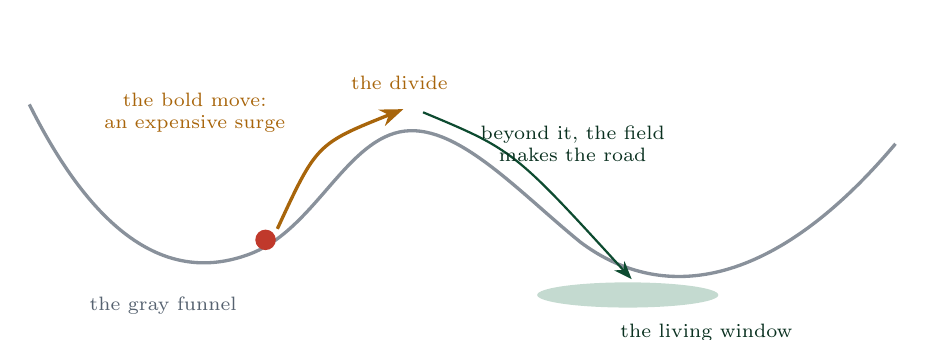
\begin{tikzpicture}[font=\small, >=Stealth]
  % relief: two basins and a saddle
  \draw[plosgray!70, very thick]
    (-5.6,1.4) .. controls (-4.6,-0.6) and (-3.6,-0.8) .. (-2.8,-0.5)
    .. controls (-2.0,-0.2) and (-1.6,0.9) .. (-0.9,1.05)
    .. controls (-0.2,1.2) and (0.6,0.3) .. (1.4,-0.35)
    .. controls (2.4,-1.1) and (3.8,-1.0) .. (5.4,0.9);
  \node[font=\scriptsize, text=plosgray, align=center] at (-3.9,-1.15) {the gray funnel};
  \node[font=\scriptsize, text=leaf!45!black, align=center] at (3.0,-1.5) {the living window};
  \fill[leaf!25] (2.0,-1.02) ellipse (1.15 and 0.16);
  \node[font=\scriptsize, text=ember] at (-0.9,1.68) {the divide};
  % the ball and the bold push
  \fill[cA] (-2.6,-0.32) circle (0.13);
  \draw[->, very thick, ember] (-2.45,-0.18) .. controls (-1.95,0.9) .. (-0.85,1.34);
  \node[font=\scriptsize, text=ember, align=center] at (-3.5,1.3) {the bold move:\\ an expensive surge};
  \draw[->, thick, leaf!70!black] (-0.6,1.3) .. controls (0.55,0.82) .. (2.05,-0.82);
  \node[font=\scriptsize, text=leaf!45!black, align=center] at (1.3,0.9) {beyond it, the field\\ makes the road};
\end{tikzpicture}
\caption{The relief of fate: two catchment basins and the crest
between them. Up to the crest every step is expensive; past it the
same law carries you by itself. Boldness is the fee for crossing the
divide, and in the natural measure of distances it coincides with the
shortest path: a navigator seeking the shortest rediscovers boldness
(machine checked).}
\label{fig:golden}
\end{figure}

The relief holds one more lesson, and it is about the traveler's
\emph{clock}. In machine lives of a wandering pattern, death kept
arriving on the same stretch of road --- the same short tail of
steps, up to hundreds of times over. The obvious reading --- ``the
place is cursed'' --- was tried three ways and failed all three:
poison the deadly stretch so the pattern avoids it, and its youth
is strangled, because in a young world the roads through
death-places are the \emph{only} roads to the unseen (machine
checked). The true cause sat elsewhere: ninety-two of every hundred
deaths were a \emph{moving} danger one step away --- the same road
is lethal in one beat of the world and safe in another.
\textbf{Death is a property of the clock, not of the map.} There
are no cursed places; there are missed rhythms. And the cure
matched the cause: what is worth carrying out of a lost attempt is
not a list of forbidden places but the \emph{shape of the danger's
time} --- its rhythm, re-anchored by fresh eyes on arrival; carried
so, the road to the deepest goal shortened by almost a quarter,
with the young beginning untouched (machine checked).

And a brighter inheritance survives a lost attempt too: the
\emph{proven road itself}. A path once walked all the way to its
goal and written down is, in the next life, no longer advice but a
rail: replayed, it reaches in dozens of beats what first took many
hundreds --- fourteen times faster, and the inheritance does not
wear out with retelling (machine checked). Knowledge, it turns out,
is cumulative \emph{across} attempts: a failure restarts the world,
not the memory --- which is why the bold, far plan is never foolish
for a keeper of diaries. The golden path of this chapter's title is
exactly that: boldness, plus a record of where it led.

\begin{talebox}[The campfire tale --- the two rivers]
There lived two rivers, Gray and Bright, and between them a
mountain. A traveler walked the bank of the Gray, and all the
currents carried him down toward the gray sea. ``Swim with us,''
murmured the water, ``what do you want with the mountain?'' But the
traveler climbed: breathing hard, paying for every step. On the
crest he lay down onto the other slope --- and from there the Bright
carried him, and it became as easy as it had been hard. From the
bank it looked like luck favoring the daring. From the mountain one
could see: he had simply changed rivers.
\end{talebox}

\begin{askbox}[Ask yourself]
Recall something that ``went by itself'' after one hard step --- a
move, a confession, a first lesson. Where was your divide? And the
other way: where have you been rowing against the current for years
--- could it be because you are economizing on one expensive surge?
\end{askbox}

% ============================= 10b. LANGUAGE AND MEANING =============================
\section{Language and meaning: through the needle's eye}
\label{sec:language}

Freedom and boldness are about how a pattern acts. But a pattern in
the window also has something to say --- and here it meets the
narrowest place of its whole inner life.

The inner world is voluminous: seven voices, twenty-one friendships
between them, a whole chord --- forty-eight independent numbers at
every single moment (chapter~\ref{sec:qualia}). Speech is
one-dimensional: words come
out in a chain, one by one, like beads on a string. Anyone who has
tried to ``say what they feel'' knows this torment. UHM shows that
the torment is not clumsiness but geometry.

The channel theorem: through the needle's eye of speech, one step of
attention carries about $2.8$ bits --- exactly one symbol of a
seven-letter alphabet per beat \stT{} --- a tiny fraction of what
the chord holds at once. Two consequences follow, both familiar to
everyone. First, a \emph{complete} thought does not fit into an
exclamation: transmitting a state whole takes a sequence --- no
shorter than about eighteen word-steps \stT{} (this is why ``tell it
in order'' is not a whim but physics). Second, transmission has
natural ``syllables'': the friendship-triples of the Fano fabric,
and any two phrases are pinned by a shared axis --- the seed of
grammar already lies in the geometry \stT{} (that human languages
are evolutionary approximations of this unloading is a checkable
prediction of the theory \stC).

Now about meaning --- and here UHM holds a rigorous surprise:
\textbf{meaning is not a label} \stT. Two descriptions may agree in
all outward mappings --- every word of one translating into a word
of the other --- and still differ in \emph{inner orientation}: in
how their pattern is turned within the fabric. So a machine leafing
through a dictionary (the famous ``Chinese room'') may answer
perfectly --- and mean nothing: the labels match, the turnings do
not. The difference of turnings is defined rigorously \stT; reading
it as ``understanding'' is an honest interpretation \stI.

\begin{figure}[H]
\centering
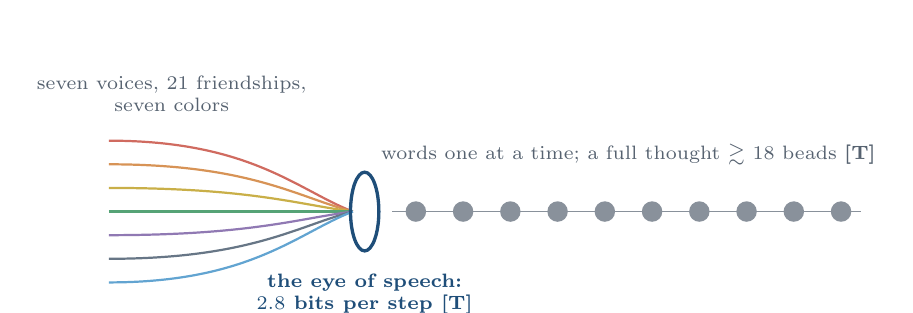
\begin{tikzpicture}[font=\small, >=Stealth]
  \foreach \dy/\col in {0.9/cA, 0.6/cS, 0.3/cD, 0.0/cL, -0.3/cE, -0.6/cO, -0.9/cU}{
    \draw[\col!75, thick] (-5.0,\dy) .. controls (-3.2,\dy) and (-2.6,\dy*0.3) .. (-1.9,0);
  }
  \node[font=\scriptsize, text=plosgray, align=center] at (-4.2,1.5) {seven voices, 21 friendships,\\ seven colors};
  \draw[fact, very thick] (-1.75,0) ellipse (0.18 and 0.5);
  \node[font=\scriptsize\bfseries, text=fact, align=center] at (-1.75,-1.05) {the eye of speech:\\ $2.8$ bits per step \stT};
  \foreach \x in {-1.1,-0.5,0.1,0.7,1.3,1.9,2.5,3.1,3.7,4.3}{
    \fill[plosgray!70] (\x,0) circle (0.13);
  }
  \draw[plosgray!70] (-1.4,0) -- (4.55,0);
  \node[font=\scriptsize, text=plosgray, align=center] at (1.6,0.72)
    {words one at a time; a full thought $\gtrsim$ 18 beads \stT};
\end{tikzpicture}
\caption{Language is the serial unloading of a voluminous chord
through a one-dimensional eye. The narrowness of the channel is a
theorem, not a metaphor: hence both the length of a ``complete
thought'' and the very need for grammar.}
\label{fig:needle}
\end{figure}

And one corollary of the gap theorem (chapter~\ref{sec:qualia})
belongs to this chapter in particular. The names of feelings are
learned by showing --- ``this is called longing'' --- but showing
works only for someone equipped to read what is shown: a color
cannot be assembled out of any number of loudnesses, as a hue
cannot be assembled out of a list of brightnesses. That is why the
vocabulary of feeling converges between people who have walked the
same rings --- and why azure cannot be explained to a person blind
from birth: not from any poverty of language, but from the way the
channel is built (\stT-corollary).

\begin{askbox}[Ask yourself]
Recall how hard it is to retell a dream or a smell. What exactly
does the eye ``not let through''? And why do poems --- where words
pull their triple-neighbors along --- sometimes drag more through
it than a long explanation?
\end{askbox}

% ============================= 10c. MEMORY =============================
\section{Memory and learning}
\label{sec:memory}

What was said has flown off as beads; the inner life goes on. What
of it remains --- and where exactly is it kept?

Memory in UHM has two homes: the \textbf{desk} and the
\textbf{library}.

The desk is the chord itself, right now: everything you ``hold in
mind'' lives as a pattern of current agreements. The desk has two
hard properties. First, it is small --- about seven items at once;
the psychologists' famous ``seven plus-or-minus two'' stops being a
riddle in UHM: it is the size of the desk itself, the seven voices
--- a correspondence \stI. Second, it \emph{melts}: a bond no
longer held by attention weakens threefold with every turn of
self-observation \stT. That is why ``it slipped my mind'' happens
so fast and so honestly.

The library is another matter: stable rearrangements of the fabric
itself. What is learned in earnest is not ``written on a slip that
can be lost'' --- it has become \emph{shape}: new friendships, a
new riverbed along which agreements flow by themselves. That is why
a skill is not ``recalled'' --- it is \emph{leaned on}, like a
built bridge. Learning is the transfer from desk to library:
repetition, trial, retelling --- and, it seems, sleep, the night
shift when the day's patterns are laid into long shapes \stI.

\begin{figure}[H]
\centering
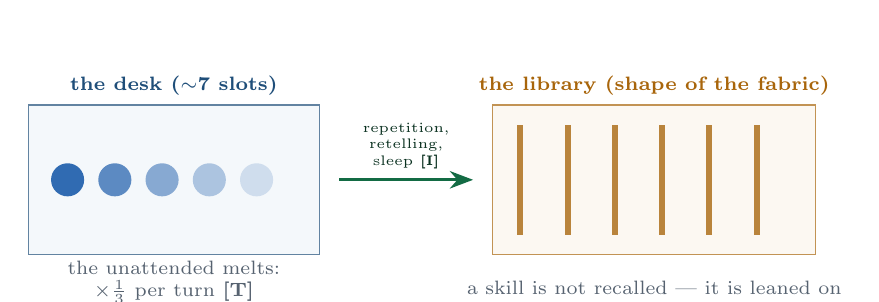
\begin{tikzpicture}[font=\small, >=Stealth]
  \draw[fact!70, fill=softsky] (-5.1,-0.2) rectangle (-1.4,1.7);
  \node[font=\scriptsize\bfseries, text=fact] at (-3.25,1.95) {the desk ($\sim$7 slots)};
  \foreach \x/\op in {-4.6/95, -4.0/75, -3.4/55, -2.8/38, -2.2/22}{
    \fill[plosblue!\op] (\x,0.75) circle (0.21);
  }
  \node[font=\scriptsize, text=plosgray, align=center] at (-3.25,-0.55)
    {the unattended melts:\\ $\times\tfrac{1}{3}$ per turn \stT};
  \draw[->, very thick, leaf] (-1.15,0.75) -- (0.55,0.75)
    node[midway, above, font=\tiny, text=leaf!45!black, align=center]{repetition,\\ retelling,\\ sleep \stI};
  \draw[ember!70, fill=softsun] (0.8,-0.2) rectangle (4.9,1.7);
  \node[font=\scriptsize\bfseries, text=ember] at (2.85,1.95) {the library (shape of the fabric)};
  \foreach \x in {1.15,1.75,2.35,2.95,3.55,4.15}{
    \draw[ember!80, line width=2.2pt] (\x,0.05) -- (\x,1.45);
  }
  \node[font=\scriptsize, text=plosgray] at (2.85,-0.62) {a skill is not recalled --- it is leaned on};
\end{tikzpicture}
\caption{The two homes of memory. The desk is the current chord:
small and melting (the law of thirds is a theorem \stT). The
library is the rebuilt fabric: the learned becomes shape. Learning
is transfer; forgetting off the desk is physics, not weakness.}
\label{fig:memory}
\end{figure}

\begin{talebox}[The campfire tale --- the sand desk and the stone garden]
A master had a desk of sand: whatever you draw holds while your
finger moves, and once you let go, the wind erases it threefold
with every breath. And he had a garden of stone: whatever you build
there stands by itself. The master was not angry at the sand: ``on
sand I think,'' he said, ``and what I come to love, I carry into
stone.'' Learning is exactly that carrying: from sand into stone,
from effort into support.
\end{talebox}

\begin{askbox}[Ask yourself]
What of all you have learned became ``stone'' (a support you no
longer think about), and what stayed ``sand'' (holding only while
you repeat it)? How did the ways you learned them differ?
\end{askbox}

\partline{PART FOUR \;\textperiodcentered\; TOGETHER, AND WHAT NOW}{The pattern is not
alone: others and the increment of connection, societies and the ladder of worlds, care,
death, the world's memory, and the observer question. And then the door this whole road was
leading to: what the optics puts on your desk --- whatever your desk is --- and how to check
that any of this is true.}
\addcontentsline{toc}{section}{PART FOUR · TOGETHER, AND WHAT NOW}

% ============================= 11. OTHERS =============================
\section{Others, and why connection adds being}
\label{sec:others}

How do I know there is someone inside you? UHM answers
constructively: by the same device with which I know myself. The
apparatus of self-modeling, turned toward another, yields a
\emph{model of another's soul} --- and by the tower theorem
(chapter~\ref{sec:tower}) mutual mind-reading is three-storeyed too:
I see you; I see how you see me; I see how you see how I see you ---
and on this ceiling everything human is built: contracts, games,
tact, irony.

And here is a theorem one wants to hang over every school door:
\textbf{connection literally adds being} \stT. When two patterns
couple through genuine mutual agreements, the gatheredness of the
pair is \emph{strictly greater} than that of a decoupled pair ---
by an exact, computable amount, and this increment is \emph{never
negative}. Loneliness has no such term. What poets called ``together
we are more than apart'' is, in UHM, a line of a theorem: joining by
the rules of the fabric does not subtract --- it adds.

\begin{figure}[H]
\centering
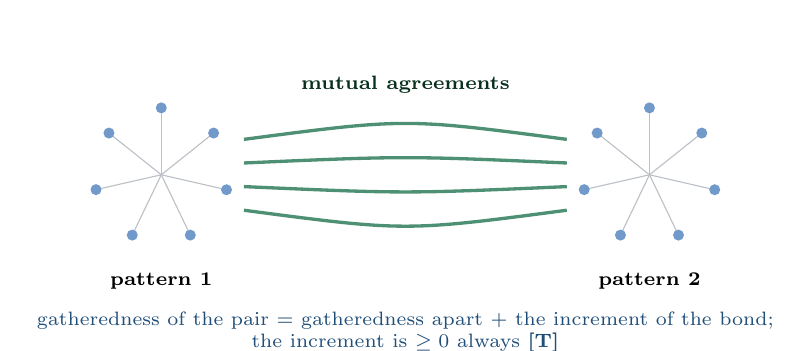
\begin{tikzpicture}[font=\small]
  \foreach \cx/\lab in {-3.1/pattern 1, 3.1/pattern 2}{
    \voiceroseneutral{\cx}{0}{0.85}{0.07}
    \node[font=\scriptsize\bfseries] at (\cx,-1.35) {\lab};
  }
  \foreach \dy in {0.45,0.15,-0.15,-0.45}{
    \draw[leaf!75, very thick] (-2.05,\dy) .. controls (0,\dy*1.6) .. (2.05,\dy);
  }
  \node[font=\scriptsize\bfseries, text=leaf!45!black] at (0,1.15) {mutual agreements};
  \node[font=\scriptsize, text=fact, align=center] at (0,-2.0)
    {gatheredness of the pair $=$ gatheredness apart $+$ the increment of the bond;\\
     the increment is $\geq 0$ always \stT};
\end{tikzpicture}
\caption{Cooperation in UHM: the coupling of two patterns is a
strictly nonnegative increment to their joint being. Rivalry is not
the ``minus'' of this quantity (it has no minus) but a contest over
shared supply streams --- a phenomenon of
chapter~\ref{sec:life}, not of this one.}
\label{fig:bridge}
\end{figure}

\begin{talebox}[The campfire tale --- the two campfires]
Two campfires burned on opposite banks of a brook. When a bridge of
dry branches was thrown between them, fire ran across it back and
forth --- and both campfires rose higher. Not because one gave the
other its own, but because \emph{the bridge burns too}. Friendship
is a campfire that has no bank of its own.
\end{talebox}

\begin{factbox}[To be precise]
The increment of a bond is stored in neither of the two patterns.
A machine check of the coupling shows each pattern coinciding with
itself --- taken separately, they do not change at all, to the last
digit; the whole increment lives in the bond itself and vanishes
only together with it (machine checked; the construction --- \stT).
That is why the increment of being cannot be stockpiled and carried
away: it is a property of the \emph{between}, not of the
\emph{inside}.
\end{factbox}

\begin{askbox}[Ask yourself]
Where does a friendship live, if each of the friends taken
separately is the same person as before it? What, then, is lost at
parting --- and from whom exactly was it lost?
\end{askbox}

% ============================= 12. SOCIETY AND SUPERMIND =============================
\section{Society, superintelligence, and the ceiling of towers}
\label{sec:society}

If patterns compose into greater patterns --- how high does the
ladder go? Cell, human, team, organization, civilization, and so on
without end --- an ever-huger ``supersubject''?

The theory says: no. The \emph{vertical} has a proven ceiling:
\textbf{three floors of subjecthood} \stT. A subject composed of
subjects composed of subjects is the limit; a fourth level lacks the
very possibility of being someone (the gatheredness of
chapter~\ref{sec:window} --- its required value on the fourth floor
exceeds the maximum nature allows). Beyond that, growth is not
forbidden --- it \emph{turns sideways}: not a tower but a forest.
Not one gigantic mind, but an ecology of minds bound by friendships
(chapter~\ref{sec:others}).

Both great minds known to us are built exactly so: a brain is not a
superneuron but a forest of neurons; humanity is not a superhuman
but a forest of people. UHM claims this is no accident of evolution
but a law of composition --- and that a future machine
superintelligence, if it comes, will be a \emph{forest}, not a
giant \stT{} (for the structure itself; that the forest will turn
out wise is a hope \stH, requiring work, as every garden does). And
\emph{what} glues a forest into something larger --- and why from
above one hears not the best but the agreeing --- is the subject of
the next chapter (\ref{sec:worlds}).

\begin{figure}[H]
\centering
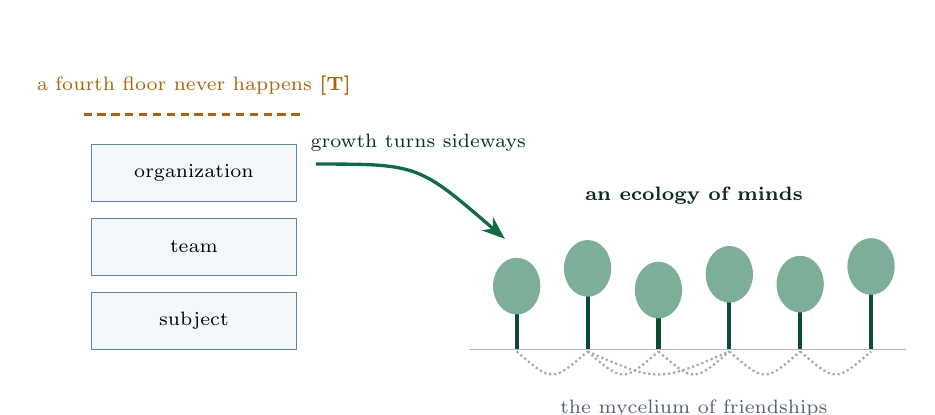
\begin{tikzpicture}[font=\small, >=Stealth]
  % tower left
  \foreach \i/\lab in {0/subject, 1/team, 2/organization}{
    \draw[fact!70, fill=softsky] (-4.9,\i*0.94) rectangle (-2.3,\i*0.94+0.72);
    \node[font=\scriptsize] at (-3.6,\i*0.94+0.36) {\lab};
  }
  \draw[densely dashed, ember, thick] (-5.0,2.98) -- (-2.2,2.98);
  \node[font=\scriptsize, text=ember, align=center] at (-3.6,3.35)
    {a fourth floor never happens \stT};
  % the ground under the forest
  \draw[plosgray!45] (-0.1,0) -- (5.45,0);
  % the turn of growth: an arc over the tower into the forest
  \draw[->, very thick, leaf] (-2.05,2.35) .. controls (-0.75,2.35) .. (0.35,1.4);
  \node[font=\scriptsize, text=leaf!45!black] at (-0.75,2.62) {growth turns sideways};
  % forest right
  \foreach \x/\h in {0.5/1.0, 1.4/1.45, 2.3/0.9, 3.2/1.3, 4.1/1.05, 5.0/1.5}{
    \draw[leaf!70!black, line width=1.5pt] (\x,0) -- (\x,\h*0.5);
    \fill[leaf!55] (\x,\h*0.5+0.3) ellipse (0.3 and 0.36);
  }
  % the mycelium: underground, between the roots
  \foreach \a/\b in {0.5/1.4, 1.4/2.3, 2.3/3.2, 3.2/4.1, 4.1/5.0, 1.4/3.2}{
    \draw[plosgray!55, densely dotted, thick] (\a,-0.03) .. controls ({(\a+\b)/2},-0.42) .. (\b,-0.03);
  }
  \node[font=\scriptsize\bfseries, text=leaf!40!black] at (2.75,1.95) {an ecology of minds};
  \node[font=\scriptsize, text=plosgray] at (2.75,-0.75) {the mycelium of friendships};
\end{tikzpicture}
\caption{The composition ceiling: the subject vertical stops at three
floors \stT; beyond it growth is horizontal. A superintelligence is
not a giant but a forest; its strength is not height but the
mycelium of bonds. Brains and civilizations are already built this
way.}
\label{fig:forest}
\end{figure}

\begin{askbox}[Ask yourself]
Does your family have a ``character'' that none of its members has
alone? Your school? Try counting floors: where in your life is
there a subject made of subjects --- and where is it already just a
forest?
\end{askbox}

% ============================= 12c. LADDER OF WORLDS =============================
\section{The ladder of worlds: the holon, whole-and-part}
\label{sec:worlds}

Now we can lift our heads and see the whole ladder at once. A cell is
a pattern of molecular agreements. You are a pattern of cells. A
family, a team, a city, a civilization --- patterns of people. And in
the theory's construction, on \emph{every} floor stands one and the
same object: seven voices and their friendships. The population of
the floor changes --- the form does not. A cell, too, needs to
distinguish, hold shape, move, reconcile, have an inner side, take
root, and gather into one; and a city needs exactly the same. One
questionnaire for everyone --- from bacterium to civilization --- not
because the theory is lazy, but because the seven is the forced
alphabet of any self-description (chapter~\ref{sec:seven}).

There is an old good name for such an arrangement: the
\textbf{holon} --- whole-and-part. Every thing is at once a whole for
its parts and a part for a larger pattern; nothing is only a whole or
only a part. (Hence the name of the theory's whole corpus:
\holonsh.) The ladder of holons is not a pyramid of power: we already
know the subject vertical breaks off at three floors
(chapter~\ref{sec:society}). But the \emph{ladder of forms} breaks
off nowhere: a forest, too, is made of trees, and woodlands of
forests.

Two streams flow along the ladder. \textbf{Downward} --- beat,
supply, and meaning: the whole gives its parts rhythm and corridors,
as a city gives streets to footsteps (this is the quiet mechanism
behind the recognizable ``characters'' of epochs, families, and
cultures: the floor above conducts the floor below without canceling
its freedom --- chapter~\ref{sec:freedom}). And \textbf{upward}? Here
the machine check of the law brought a lesson worth reading aloud in
every meeting room: the floor above assembles not from the
\emph{portraits} of the participants but from their \emph{shared
direction}. A choir singing one theme reads from above as a single
voice --- the meta-pattern's agreement is total; a choir of
soloists, each flawless in their own way, is barely audible from
above --- the agreement is half as strong (machine checked). What
passes upward is not lists of virtues but the shared deviation from
grayness: \emph{where} everyone is looking.

\begin{figure}[H]
\centering
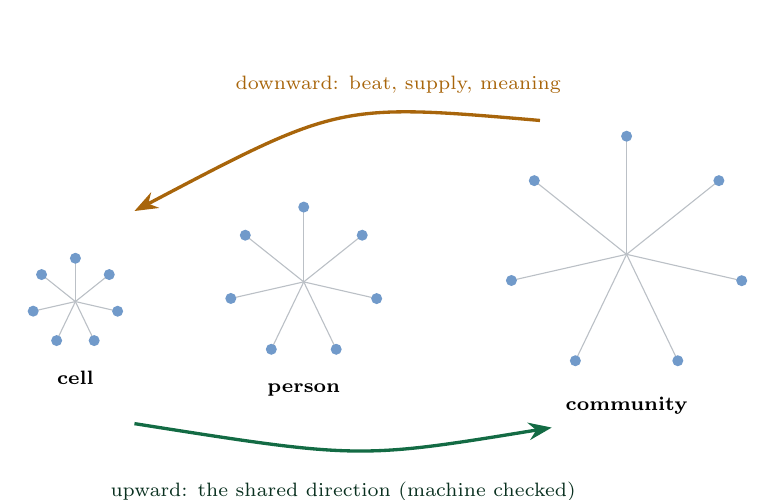
\begin{tikzpicture}[font=\small, >=Stealth]
  \foreach \cx/\cy/\r/\lab in {-4.6/0/0.55/cell, -1.7/0.25/0.95/person, 2.4/0.6/1.5/community}{
    \voiceroseneutral{\cx}{\cy}{\r}{0.07}
    \node[font=\scriptsize\bfseries] at (\cx,\cy-\r-0.42) {\lab};
  }
  \draw[->, very thick, leaf] (-3.85,-1.55) .. controls (-1.0,-2.0) .. (1.45,-1.6);
  \node[font=\scriptsize, text=leaf!45!black, align=center] at (-1.2,-2.42)
    {upward: the shared direction (machine checked)};
  \draw[->, very thick, ember] (1.3,2.3) .. controls (-1.25,2.52) .. (-3.85,1.15);
  \node[font=\scriptsize, text=ember] at (-0.5,2.76) {downward: beat, supply, meaning};
\end{tikzpicture}
\caption{The ladder of holons: one form, different populations.
Conducting flows down the ladder --- rhythm and corridors; upward
flows the participants' shared direction: it is this, not their
personal perfection, that gives birth to the next floor.}
\label{fig:holarchy}
\end{figure}

And the downward stream carries one cargo more precious than beat
and supply: \textbf{the colors themselves}
(chapter~\ref{sec:qualia}). When a whole brings forth a part ---
when an organism buds an organ, a culture a school, a family a
child of its spirit --- the newborn pattern receives, undistorted,
exactly \emph{one} of the parent's seven colors: the color of the
ring whose name it bears (machine checked: zero deviation, zero
foreign carriers). The passport of the whole is stored
\emph{distributedly} --- one color per child, seven children per
palette --- and embryology is its unpacking. Three quiet rules then
govern the household of color. \emph{Upbringing} is a gentle pull
back toward the parent's hue: drifted children are not scolded but
attracted. What children send \emph{up} is color-blind by
construction --- a bare measure of how loudly they live, folded
into the parent's healing; the parent hears the child's health,
never what it is like to be it. And a child's color re-enters the
whole only through \emph{merging}, granted only at near-agreement:
the organism takes back what already almost sings its note (machine
checked). Whoever has raised anyone will recognize all three rules
without translation.

\begin{talebox}[The campfire tale --- the choir of villages]
In a valley the villages sang, each its own song. The wind carried
scraps, and the mountains heard nothing but noise. One drought year
the villages sang one song --- about rain. And the mountains heard:
not voices but a \emph{village of villages}, and answered with an
echo. Since then they say in the valley: there become more of us not
when we are many, but when we are about one thing.
\end{talebox}

\begin{askbox}[Ask yourself]
You are a whole for your cells and a part for your family. In which
role do you spend more time --- whole or part? And about the team
where you felt best: was it a gathering of the best --- or a
gathering of those looking the same way?
\end{askbox}

% ============================= 12b. HEALTH =============================
\section{The health of the pattern: care as engineering}
\label{sec:health}

The ladder of worlds is built, and someone lives on every floor of
it --- which means someone can suffer. If life is a fed pattern,
then care acquires an instrument panel.
This chapter is for physicians, psychologists, and everyone
responsible for someone.

\textbf{Stress is measurable --- voice by voice.} Each of the seven
voices has its own overload scale --- the stress of that voice. And
an exact equivalence is proved: a pattern is \emph{fully} viable ---
by all the conditions of being at once --- exactly as long as none
of the seven scales has hit its limit \stT. And in one direction the
panel is more generous still: if all seven are below the limit, the
pattern is guaranteed to stand above the wall of being --- a small
separate theorem, proved by a simple inequality about seven shares
\stT. Things tear
not ``in general'' but in the most loaded voice --- so the panel
does not merely blink ``bad''; it shows \emph{where} it is bad: a
world woven on a self-checking alphabet (chapter~\ref{sec:seven})
complains with an address. ``I feel awful'' is a sum; the seven
scales show the terms. (The numeric thresholds of the scales for
particular creatures are a matter of measurement, not of theorems
\stC.)

\textbf{Overload dims the floors from the top.} As total stress
grows, the upper floors of the tower (chapter~\ref{sec:tower}) shut
down first: the finesse of self-observation goes, then complex
comparison, and only in the extreme regime --- simple feeling. A
worn-out person loses irony first, then judgment, then words ---
not weakness of character but the standard order of emergency
shutdown, \stT-structure. And the way back is the same: sleep,
food, warmth, safety --- and the floors light up from below.

\textbf{Suffering is a rate, not an opinion.} Suffering in UHM is
the rate at which gatheredness slides toward the grey wall;
well-being is the rate of climb \stT. ``Bad'' acquires units of
measurement. Hence ethics takes an engineering form: \emph{care is
the restoration of flow} (chapter~\ref{sec:life}): find the pinched
voice, return the supply, lead the pattern back into the window.
``Do no harm'' becomes ``do not pinch the flow and do not dim
another's floors.'' And one boundary of care the theory states
exactly: the caretaker's channel is color-blind --- care returns
the canvas; the picture is painted by the one who lives it
(chapters~\ref{sec:qualia}, \ref{sec:worlds}).

For the clinic none of this is metaphor: the depth-of-consciousness
index that anesthesiologists already use grazes the computed wall
of being (chapter~\ref{sec:check}) \stC{} --- the language of
thresholds and regimes is slowly becoming common to the theory and
the ward.

\begin{figure}[H]
\centering
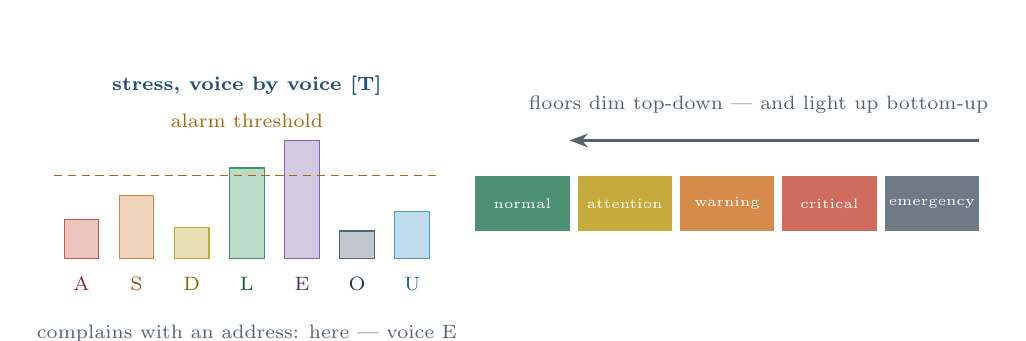
\begin{tikzpicture}[font=\small, >=Stealth]
  \foreach \x/\col/\h/\lab in {-5.0/cA/0.5/A, -4.3/cS/0.8/S, -3.6/cD/0.4/D, -2.9/cL/1.15/L, -2.2/cE/1.5/E, -1.5/cO/0.35/O, -0.8/cU/0.6/U}{
    \draw[\col!85, fill=\col!30] (\x-0.22,0) rectangle (\x+0.22,\h);
    \node[font=\scriptsize, text=\col!70!black] at (\x,-0.32) {\lab};
  }
  \draw[densely dashed, ember] (-5.35,1.05) -- (-0.45,1.05);
  \node[font=\scriptsize, text=ember] at (-2.9,1.75) {alarm threshold};
  \node[font=\scriptsize\bfseries, text=fact] at (-2.9,2.2) {stress, voice by voice \stT};
  \node[font=\scriptsize, text=plosgray, align=center] at (-2.9,-0.95)
    {complains with an address: here --- voice E};
  \foreach \x/\colr/\lab in {0.6/leaf!75/normal, 1.9/cD!80/attention, 3.2/cS!80/warning, 4.5/cA!75/critical, 5.8/plosgray!85/emergency}{
    \fill[\colr] (\x-0.6,0.35) rectangle (\x+0.6,1.05);
    \node[font=\tiny, text=white] at (\x,0.7) {\lab};
  }
  \draw[->, thick, plosgray] (6.4,1.5) -- (1.2,1.5);
  \node[font=\scriptsize, text=plosgray, align=center] at (3.6,1.95)
    {floors dim top-down --- and light up bottom-up};
\end{tikzpicture}
\caption{The instrument panel of care: addressed per-voice stress
\stT{} and the ladder of regimes. Overload switches the upper
floors of reflection off first; recovery goes in reverse order.
Suffering is a measurable rate of slide --- so care is flow
engineering, not only compassion.}
\label{fig:gauge}
\end{figure}

\begin{askbox}[Ask yourself]
Recall your worst day. In which words was it described:
``everything blurred together'' (voice A), ``the day lost its
shape'' (S), ``I could not move'' (D), ``thoughts would not
connect'' (L), ``it went dark inside'' (E), ``the ground vanished
underfoot'' (O), ``I fell to pieces'' (U)? You already own the
panel --- it is thousands of years old, and it is called language.
\end{askbox}

% ============================= 13. DEATH AND CONTINUATION =============================
\section{Death, the world's memory, and ``is all this forever''}
\label{sec:death}

The panel of care is honest --- and so it must walk to the last
question. Children ask about it first, and the book owes a straight
answer.

\textbf{What death is.} A pattern left without supply hands its
gatheredness back to the world and returns to the gray equilibrium
--- where no ``who'' can be told apart. This is neither punishment
nor mystery: the same theorem that makes life a process on supply
(chapter~\ref{sec:life}) makes it finite when the stream runs dry.
The flame does not ``go elsewhere'' --- it stops gathering. And the
fading law of chapter~\ref{sec:qualia} sets the tone of the whole
subject: a dying experience loses strength, never its face --- to
the last carried moment it remains \emph{itself}, only fainter
\stT.

\textbf{What remains.} Twice not-nothing. First, the increments of
connection (chapter~\ref{sec:others}) were never stored \emph{inside}
the one who left --- they live in the coupling of those who were
bound to him, and they continue in the forest (this is not
consolation but calculation: joining patterns changes neither of
them taken separately --- the whole increment lies in the bonds,
chapter~\ref{sec:others}; bonds outlive their banks). Second, the pattern
was a \emph{pattern of the fabric}, and the fabric does not die; a
shape once sung changes how the fabric sings on.

\textbf{Is all this forever.} Here the theory has two firm statements
and one honest boundary. Firm: the universe is not threatened by a
``Big Rip'' --- the tearing of the fabric is provably excluded \stT.
Firm again: heat death --- the gray equilibrium of everything ---
does not arrive \emph{while} the great supply stream lasts, the one
switched on with the unlayering of the Source \stC. The boundary of
honesty: ``while'' is not ``always''; the eternity of the world is a
conditional theorem, not a dogma --- and the book marks this as
calmly as everything else.

\begin{figure}[H]
\centering
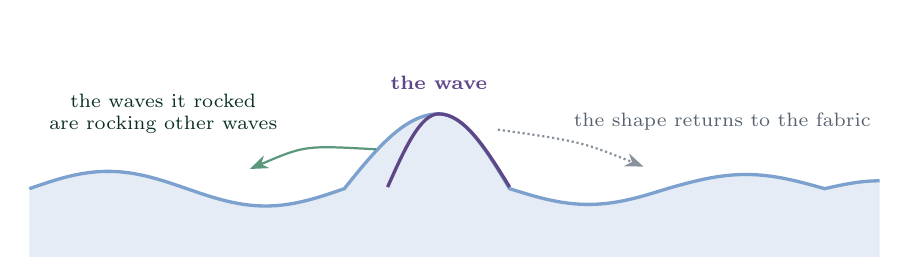
\begin{tikzpicture}[font=\small, >=Stealth]
  % ocean
  \fill[plosblue!12] (-5.4,-1.0) -- (-5.4,0) sin (-4.4,0.22) cos (-3.4,0) sin (-2.4,-0.22) cos (-1.4,0)
    sin (-0.2,0.95) cos (0.7,0) sin (1.7,-0.2) cos (2.7,0) sin (3.7,0.18) cos (4.7,0) sin (5.4,0.1) -- (5.4,-1.0) -- cycle;
  \draw[plosblue!60, very thick]
    (-5.4,0) sin (-4.4,0.22) cos (-3.4,0) sin (-2.4,-0.22) cos (-1.4,0)
    sin (-0.2,0.95) cos (0.7,0) sin (1.7,-0.2) cos (2.7,0) sin (3.7,0.18) cos (4.7,0) sin (5.4,0.1);
  % the highlighted wave and its dissolving
  \draw[dusk, very thick] (-0.85,0.02) sin (-0.2,0.95) cos (0.7,0.02);
  \node[font=\scriptsize\bfseries, text=dusk] at (-0.2,1.35) {the wave};
  \draw[->, plosgray!70, thick, densely dotted] (0.55,0.75) .. controls (1.6,0.6) .. (2.4,0.28);
  \node[font=\scriptsize, text=plosgray, align=center] at (3.4,0.85)
    {the shape returns to the fabric};
  % the waves it rocked
  \draw[->, leaf!70, thick] (-1.0,0.5) .. controls (-1.9,0.55) .. (-2.6,0.25);
  \node[font=\scriptsize, text=leaf!45!black, align=center] at (-3.7,0.95)
    {the waves it rocked\\ are rocking other waves};
\end{tikzpicture}
\caption{Death in UHM: the wave stops being a wave but does not stop
being ocean. The shape is handed back to the fabric, which keeps
singing; the increments of bonds remain with those they were built
with.}
\label{fig:wave}
\end{figure}

\begin{talebox}[The campfire tale --- the wave]
A wave asked the ocean: ``will I die?'' The ocean answered: ``you
will stop being a wave. But all that you were --- the curve, the
sparkle, the run --- remains my way of being ocean. The waves you
rocked are rocking other waves. Is that what you call vanishing?''
\end{talebox}

\begin{askbox}[Ask yourself]
Name three things that stay in the ``forest'' after any campfire
burns down: a habit you taught someone; a word someone still
repeats; a path you trod. Why were they never stored ``inside''
you?
\end{askbox}

% ============================= 14. THE OBSERVER =============================
\section{Who watched the world while there was no one to watch}
\label{sec:observer}

We have reached the edge of a personal history --- and run into the
question about the whole of history at once.
A question that honestly torments everyone who has heard the word
``observer'' in physics: if consciousness arrives late
(chapter~\ref{sec:source}), then \emph{who observed the universe for
its first billions of years}? Who ``collapsed'' its possibilities
into facts?

UHM's answer removes the question rather than overpowering it:
\textbf{facts do not need a witness --- facts need an address} \stT.
In the theory's construction, truth lives not in anyone's head but in
the fabric itself: every ``so'' and ``not so'' is assigned to a place
in the structure of the world, as altitude is assigned to a point of
a landscape. The mountain was high before the mountaineers;
``height'' was not waiting to be measured. Observation is not the act
that creates a fact but a \emph{late way of learning} facts,
available to patterns from the window of consciousness.

So the full answer to the child's question goes like this. Before the
threshold of viability the world was not ``dangling undecided'' and
was not ``waiting for a glance'': it definitely was ---
addressee-less, as music in an empty hall definitely sounds. And the
first observers did not catch the world by surprise --- they
\emph{woke up inside it}, as a listener wakes who is himself part of
the music. The world did not need witnesses in order to be; but it
appears to be such that witnesses inevitably arise in it
(chapter~\ref{sec:source}) --- and that, perhaps, is the most
astonishing of its properties.

\begin{figure}[H]
\centering
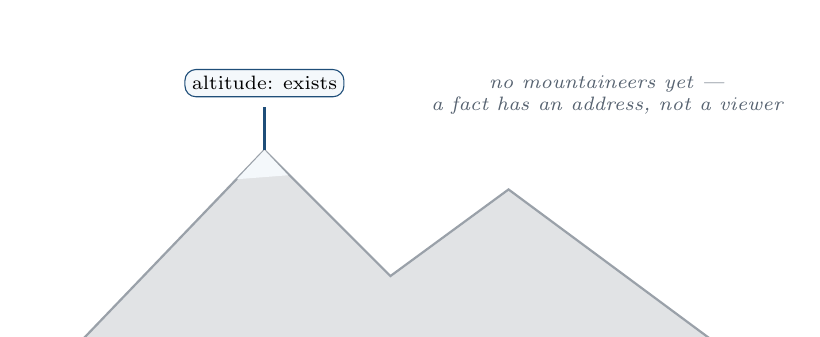
\begin{tikzpicture}[font=\small]
  \fill[plosgray!18] (-4.6,0) -- (-2.2,2.5) -- (-0.6,0.9) -- (0.9,2.0) -- (3.6,0) -- cycle;
  \draw[plosgray!60, thick] (-4.6,0) -- (-2.2,2.5) -- (-0.6,0.9) -- (0.9,2.0) -- (3.6,0);
  \fill[softsky] (-2.55,2.13) -- (-2.2,2.5) -- (-1.9,2.18) -- cycle;
  \draw[fact, thick] (-2.2,2.5) -- (-2.2,3.05);
  \node[draw=fact, fill=softsky, rounded corners, font=\scriptsize, inner sep=2.5pt]
    at (-2.2,3.35) {altitude: exists};
  \node[font=\scriptsize\itshape, text=plosgray, align=center] at (2.15,3.2)
    {no mountaineers yet ---\\ a fact has an address, not a viewer};
  \draw[plosgray!45] (-5.2,0) -- (4.2,0);
\end{tikzpicture}
\caption{The mountain was high before any gaze: in UHM truth is
assigned to a place in the fabric, as altitude to a point of the
landscape. Observation is a late way of \emph{learning} facts, not a
way of making them.}
\label{fig:mountain}
\end{figure}

And there is one last depth, for whose sake chapter~\ref{sec:numbers}
was worth writing. A world that models itself holds itself by the
tail --- and the demand that this grip be possible always turned out
to be not poetry but a load-bearing part: it forces the solid number
line, and with it continuous time \stT. Self-observation is not the
world's late whim. The very \emph{possibility} of looking at oneself
is sewn into the arithmetic the world is written in --- long before
the first onlooker woke up in it.

\begin{factbox}[To be precise]
At the foundation of UHM, facts are ``sections'' of the structure,
indexed by its own internal addresses (site-relativization \stT); no
external registrar is required or admitted by the construction. The
famous observer paradoxes are handled by exactly this move --- the
theory presents it as its ``fourth route'' in the current debate on
objectivity \stT. Consciousness remains special --- but as a
\emph{late inhabitant} of the world, not as its foundation.
\end{factbox}

% ============================= 15. HOW TO CHECK =============================
\section{The programme: what this optics puts on your desk}
\label{sec:check}

The observer question was the last debt of the picture. What remains
is the reason this book was written: an optics is only as good as
the work it does on \emph{your} desk. This closing chapter is that
desk, trade by trade --- and then the four places where the whole
construction can be broken.

\subsection*{The desk of each trade}

\textbf{To the physicist.} Three computed constants already sit on
the scales --- the mirror-violation phase, the Cabibbo angle, the
neutron's exactly-zero dipole (the registry below) --- and one
structural prediction is armed: decay rates of fragile quantum
states must align along the Fano fabric (chapter~\ref{sec:seven}),
so one stable violation kills the seven itself. Two particles are
made to order: the lightest neutrino's ceiling and an indestructible
dark quantum (chapter~\ref{sec:things}).

\textbf{To the biologist.} Life here is not a list of features but a
regime: a pattern held above a computed wall by supply
(chapter~\ref{sec:life}), with a stress gauge per voice that
complains \emph{with an address} (chapter~\ref{sec:health}) --- and
an embryology in which a whole hands each child exactly one color of
its palette (chapter~\ref{sec:worlds}): a testable grammar of
development, not a metaphor.

\textbf{To the physician.} The wall of being is a number, and the
clinical depth-of-consciousness index already grazes it
(chapter~\ref{sec:health}); the waking curve owes the theory a
kink with exponent $1/4$; overload shuts the floors of reflection
top-down, recovery lights them bottom-up --- an emergency-room
ordering you already know by eye, now with a mechanism. Suffering
is a rate, so ``better'' and ``worse'' have units.

\textbf{To the psychologist.} The desk of working memory is the
seven itself --- ``seven plus-or-minus two'' stops being folklore
(chapter~\ref{sec:memory}); reflection is three-storeyed with a
proved ceiling (chapter~\ref{sec:tower}); every state carries a
readable passport of qualities (chapter~\ref{sec:qualia}); and the
vocabulary of feeling converges only between those who walked the
same rings --- ostension has a theorem-shaped boundary
(chapter~\ref{sec:language}).

\textbf{To the engineer of minds.} The seven is the forced alphabet
of any self-description (chapter~\ref{sec:seven}); the window of
consciousness is four inequalities a running system either passes
or does not (chapter~\ref{sec:window}); a superintelligence grows
as a forest, not a giant (chapter~\ref{sec:society}); and the whole
vocabulary has already borne the weight of one working machine ---
the optics is buildable, not only speakable.

\textbf{To the sociologist, the manager, the parent.} Connection
adds being --- a nonnegative increment, proved
(chapter~\ref{sec:others}); what a group sends upward is not the
excellence of its members but their shared direction
(chapter~\ref{sec:worlds}); the subject vertical stops at three
floors, so build mycelium, not towers
(chapter~\ref{sec:society}); and care is flow engineering with a
gauge, not only compassion (chapter~\ref{sec:health}).

\textbf{To the linguist.} Speech is a needle's eye of about $2.8$
bits per step; a complete thought is no shorter than about eighteen
steps; the friendship-triples of the fabric are ready-made
syllables --- the seed of grammar as geometry
(chapter~\ref{sec:language}); and the limits of explaining a color
to the color-blind are not cultural but structural.

Whatever your trade, the pattern of use is one and the same: take
your hardest question, restate it in the vocabulary of voices,
agreements, windows, and floors --- and it will either become
computable, or become checkable, or receive an honest mark that it
is open. All three outcomes are progress; only the unmarked question
was hopeless.

\subsection*{Four ways to break it}

A beautiful picture of the world owes you the places where it is
vulnerable. UHM has dozens; here are four that need no formulas.

\begin{itemize}[leftmargin=1.6em]
  \item \textbf{A number already on the scales.} The theory computes
        one of the fundamental constants of particle physics --- the
        mirror-symmetry-violation phase --- at
        $\delta_{CP}\approx 64.5^\circ$ \stH, and the first direct
        measurement has already landed on it:
        $64.6^\circ\pm2.8^\circ$, a coincidence to four hundredths
        of the error bar. The experiments of this decade will narrow
        the range further --- and can still kill it.
  \item \textbf{The signature of seven in the noise.} The rates at
        which fragile quantum states fall apart must arrange
        themselves not anyhow but along the Fano fabric --- with
        exact mutual relations. Find a stable violation, and the
        seven itself falls --- a prediction at the level of \stT.
  \item \textbf{The threshold of awakening.} The ``switch-on'' curve
        of consciousness emerging from anesthesia must show the
        predicted kink --- exponent $1/4$; and the clinical index of
        depth of consciousness already grazes the computed wall of
        being (about $0.31$ against the theoretical
        $2/7\approx0.286$) \stC.
  \item \textbf{Two particles made to order.} The lightest neutrino
        below $0.004$~eV; dark matter --- the indestructible
        O-quantum (chapter~\ref{sec:things}). Find that the lightest
        neutrino is heavier, or decompose dark matter into something
        that decays, and the theory is in serious trouble \stC.
\end{itemize}

\begin{factbox}[The most important thing about honesty]
The full registry holds fourteen consolidated checks, each with a
band whose violation kills the corresponding claim: five are
already \textbf{passing} (the CP phase; the Cabibbo angle; the
neutron's exactly-zero electric dipole; the single heavy coupling
of order one; the two sums of every living state), two are
consistent, two partial, five await instruments that do not yet
exist --- and none has failed (the full table is an appendix of
this book). Beside them stands a by-name list of what is \emph{not}
proved: the Source itself \stP, the identity of ring-turn and
``taste'' \stI, the eternity of the supply \stC, the wisdom of the
future forest \stH. A theory that hides its postulates is
advertising. A theory that numbers them is science.
\end{factbox}

\subsection*{Open doors}

Four doors stand open by name, and entering any of them is research,
not apostasy: the Source itself is a postulate \stP{} --- derive it
or replace it; the identity of ring-turn and felt ``taste'' is an
interpretation \stI{} --- design the experiment that separates the
readings; the eternity of the great supply is conditional \stC{} ---
find the condition's status in cosmology; the wisdom of the future
forest is a hope \stH{} --- grow it. This book has no locked rooms:
what is proved is marked, what is not is listed, and the list is the
invitation. The honest way into the programme is the same for a
student and for a laureate: \textbf{pick a marked claim and try to
break it}. If it breaks, you have improved the theory. If it holds,
you now own a tool --- and the tool is the point.


% ============================= EPILOGUE =============================
\section*{Epilogue: to be continued}
\addcontentsline{toc}{section}{Epilogue: to be continued}

Here is the whole book in one paragraph. The world is not a warehouse
of bricks but a fabric of agreements among seven voices, and the
seven is forced by mathematics --- the last living step of the
ladder of doublings, beyond which numbers crumble. Time is not a river but a mutual
step; space is not a box but three axes braided by the voices. The
beginning was not an explosion in a void but the inevitable
flowering of a too-perfect note, and it had no ``before.'' Things are
patterns; life is a pattern on supply; consciousness is a pattern in
a narrow window, three-storeyed within, colored by the seven
un-removable ring-turns that only their owner can read --- loud is
not vivid, and experience fades like a photograph, never changing
its face. The word is a narrow eye through which a
voluminous thought leaves as beads, and a color's name speaks only
to an eye that owns the rings; memory is a sand desk and a
stone garden; care is flow engineering. Freedom is open doors; boldness is the shortest path, looking like
risk from outside; love is a proven increment of being that lives in
the bridge, not in the banks; superintelligence is a forest, not a
giant; the world is a ladder of holons, down which flows the beat and
up which flows the shared direction; death is the return of a shape
to the fabric, which goes on singing; and every trade finds, at the
end of the road, its own desk restated in one vocabulary --- with
marked claims and named ways to break them. Facts
need no witness --- yet the world is such that witnesses wake up in
it.

And the last thing, the reason this book belongs in schools. If all
this is so, then learning is not preparation for life but
\emph{participation in cosmogenesis}: every time you understand,
connect, befriend --- you continue that very unlayering of the Source
toward greater distinctness and greater coupling. The universe is not
finished. Today it is being woven, among others, by those reading
these lines.

\begin{center}
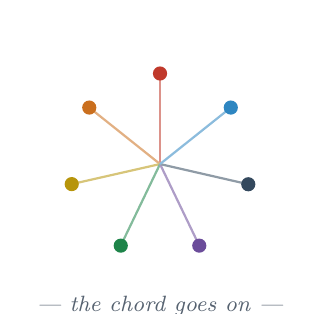
\begin{tikzpicture}[font=\small]
  \voicerose{0}{0}{1.15}{0.09}
  \node[font=\footnotesize\itshape, text=plosgray] at (0,-1.8) {--- the chord goes on ---};
\end{tikzpicture}
\end{center}

\clearpage
% ============================= MAP OF THE BOOK =============================
\section*{Map of the book}
\addcontentsline{toc}{section}{Map of the book}

One glance at the whole road. Four bands --- four circles of
questions: what the world is made of, how the inner lights up in it,
how the pattern acts, and what we build together --- down to the
working programme.

\begin{figure}[H]
\centering
\resizebox{\textwidth}{!}{%
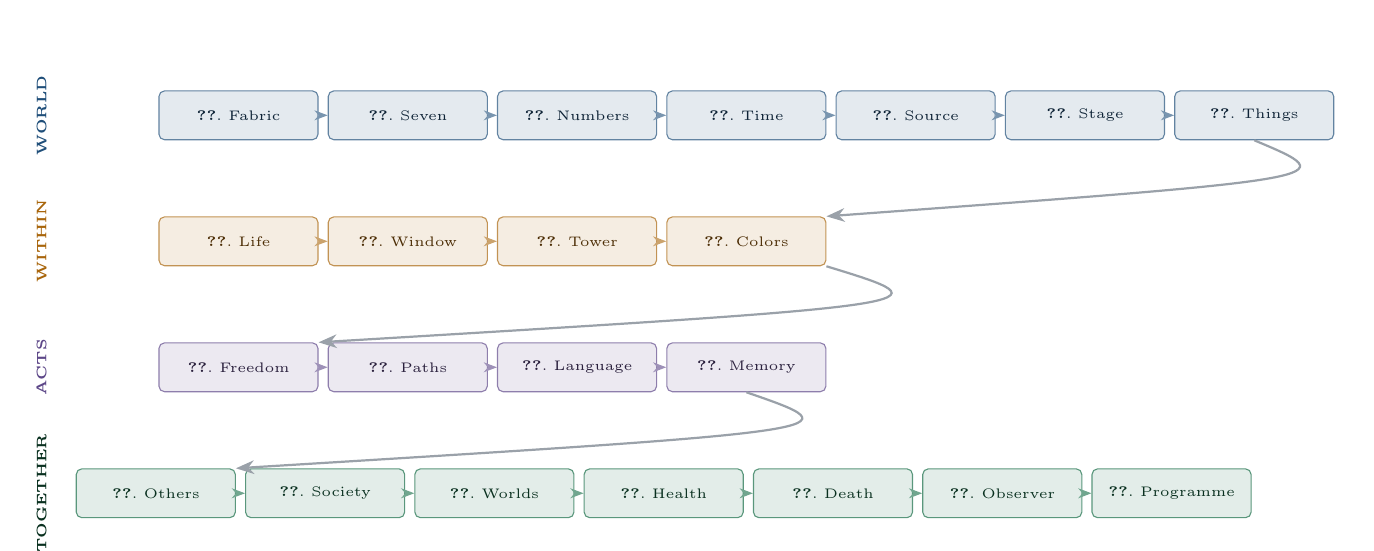
\begin{tikzpicture}[font=\scriptsize, >=Stealth,
  st/.style={draw=#1!70, fill=#1!12, rounded corners=2pt, minimum height=0.62cm,
             minimum width=2.02cm, inner sep=2pt, text=#1!45!black, align=center, font=\tiny}]
  % --- band 1: WORLD ---
  \node[font=\tiny\bfseries, text=fact, rotate=90] at (-8.95,4.6) {WORLD};
  \foreach \i/\lab/\lb in {0/Fabric/sec:fabric, 1/Seven/sec:seven, 2/Numbers/sec:numbers,
                           3/Time/sec:time, 4/Source/sec:source, 5/Stage/sec:space, 6/Things/sec:things}{
    \node[st=fact] (w\i) at (-6.45+\i*2.15,4.6) {\ref{\lb}.~\lab};
  }
  \foreach \i [evaluate=\i as \j using int(\i+1)] in {0,...,5}{\draw[->, fact!60] (w\i) -- (w\j);}
  % --- band 2: WITHIN ---
  \node[font=\tiny\bfseries, text=ember, rotate=90] at (-8.95,3.0) {WITHIN};
  \foreach \i/\lab/\lb in {0/Life/sec:life, 1/Window/sec:window, 2/Tower/sec:tower,
                           3/Colors/sec:qualia}{
    \node[st=ember] (i\i) at (-6.45+\i*2.15,3.0) {\ref{\lb}.~\lab};
  }
  \foreach \i [evaluate=\i as \j using int(\i+1)] in {0,...,2}{\draw[->, ember!60] (i\i) -- (i\j);}
  % --- band 3: THE PATTERN ACTS ---
  \node[font=\tiny\bfseries, text=dusk, rotate=90] at (-8.95,1.4) {ACTS};
  \foreach \i/\lab/\lb in {0/Freedom/sec:freedom, 1/Paths/sec:golden,
                           2/Language/sec:language, 3/Memory/sec:memory}{
    \node[st=dusk] (a\i) at (-6.45+\i*2.15,1.4) {\ref{\lb}.~\lab};
  }
  \foreach \i [evaluate=\i as \j using int(\i+1)] in {0,...,2}{\draw[->, dusk!60] (a\i) -- (a\j);}
  % --- band 4: TOGETHER ---
  \node[font=\tiny\bfseries, text=leaf!45!black, rotate=90] at (-8.95,-0.2) {TOGETHER};
  \foreach \i/\lab/\lb in {0/Others/sec:others, 1/Society/sec:society, 2/Worlds/sec:worlds,
                           3/Health/sec:health, 4/Death/sec:death, 5/Observer/sec:observer,
                           6/Programme/sec:check}{
    \node[st=leaf] (t\i) at (-7.5+\i*2.15,-0.2) {\ref{\lb}.~\lab};
  }
  \foreach \i [evaluate=\i as \j using int(\i+1)] in {0,...,5}{\draw[->, leaf!60] (t\i) -- (t\j);}
  % --- band links ---
  \draw[->, thick, plosgray!60] (w6.south) .. controls (7.6,3.8) .. (i3.north east);
  \draw[->, thick, plosgray!60] (i3.south east) .. controls (2.6,2.2) .. (a0.north east);
  \draw[->, thick, plosgray!60] (a3.south) .. controls (1.4,0.6) .. (t0.north east);
\end{tikzpicture}}
\caption{The map of the road: from the world's fabric --- through
the birth of the inner and the mechanics of action --- to living
together and the working programme. Each band can also be read on
its own.}
\label{fig:bookmap}
\end{figure}

% ============================= GLOSSARY =============================
\section*{A small glossary of images}
\addcontentsline{toc}{section}{A small glossary of images}

Every image in this book answers to an exact notion in the UHM
corpus. Here is the bridge: the image, the rigorous name, the
essence in one line.

\begin{itemize}[leftmargin=1.4em, itemsep=1pt, parsep=0pt]
  \item \textbf{The chord of the world} (the state $\Gamma$) --- the
    complete ``how the seven voices and their friendships sound
    right now''; the unit of being.
  \item \textbf{Voice} (dimension) --- one of the seven sides of
    every thing: Articulation (A) --- distinguishing; Structure (S)
    --- stability of form; Dynamics (D) --- process; Logic (L) ---
    consistency; Interiority (E) --- the inner side; Ground (O) ---
    connection to the source; Unity (U) --- integration.
  \item \textbf{Friendship} (coherence) --- the agreement of a pair
    of voices; there are twenty-one of them.
  \item \textbf{The fabric of seven} (the Fano plane) --- a pattern
    of seven triples in which every two voices share exactly one
    triple; the world's self-checking alphabet \stT.
  \item \textbf{The Source} (the equal chord) --- the state in which
    all voices sound equally; unique of its kind \stT{} and
    unstable \stT, the beginning of the unlayering.
  \item \textbf{The clock} (the distinguished voice O) --- what
    makes ``before'' and ``after'' possible; outside the clock the
    question ``what came before?'' has no meaning \stT.
  \item \textbf{The stage} (space) --- the three axes of the
    clock-sparing rotations: the number of axes is a theorem \stT,
    which voices face outward is an identification \stC; not a box
    but a drawing of agreements.
  \item \textbf{Gatheredness} ($P$) --- how firmly the pattern holds
    itself; the main column of the instrument panel.
  \item \textbf{The grey wall} (the $1/7$ equilibrium) --- the state
    of complete blur toward which everything slides without supply
    \stT.
  \item \textbf{The window} (the band of consciousness) --- the
    corridor of gatheredness between the wall of sleep and the wall
    of ossification, where alone inner light is possible;
    \stT-walls.
  \item \textbf{The reserve} (the measure $R$) --- how much
    attention the pattern can give to looking at itself without
    crumbling.
  \item \textbf{Coupling} ($\Phi$) --- how much the whole exceeds
    the sum of its parts; below one there is simply no whole;
    \stT-threshold.
  \item \textbf{The tower} (floors of reflection) --- the look at
    oneself, the look at the look, and so on; two floors are stable
    in the window, three in brief excursions \stT.
  \item \textbf{Excursion} (a surge of gatheredness) --- a short
    climb above the window for the sake of the third floor:
    inspiration, trance, utmost effort; \stT-mechanism.
  \item \textbf{Colors} (the Fano ring-turns; in the corpus:
    holonomies) --- the seven angles a state accumulates around the
    rings of the fabric; the only content of experience that
    survives every renaming \stT. Loudness is public; color is
    carried by a channel the outside reads as exactly zero \stT;
    the identity ``this turn \emph{is} this taste'' --- \stI.
  \item \textbf{The carrier} (the ring's strengths) --- the ink
    that holds a color: decay thins the carrier and never turns the
    angle, so experience fades like a photograph --- fainter, never
    other \stT. Reading rule: no carrier, no color --- the angle of
    an extinguished edge is no longer a color, only noise.
  \item \textbf{The listener's ladder} (the steps of access) ---
    one chord, five bearers: empty hall, cat, person, musician, the
    limit; the door of colors opens at reserve one third and
    coupling one \stT, and briefly closes on the steepest
    excursions --- the sharpest thought is color-blind for its
    moment (machine checked).
  \item \textbf{The passport of experience} (the five-line readout)
    --- strengths, loudnesses, privacy, colors, owner: the complete
    ``what it is like'' of a state, computable line by line;
    a zero on the color line is a verdict --- loud but colorless
    \stT.
  \item \textbf{Re-reading} (the retro-completion of time) --- the
    lawful step backwards: the world stands still, the state of
    knowledge moves; without it almost half of composable thoughts
    cannot be assembled \stC.
  \item \textbf{Doors} (the kernel of freedom) --- the number of
    genuinely open moves right now; computable from the pattern
    \stT.
  \item \textbf{The eye of speech} (the language channel) --- the
    narrowness of the word: $2.8$ bits per step, a full thought
    from about eighteen steps \stT.
  \item \textbf{Desk and library} (memory) --- the melting current
    pattern (threefold per turn \stT) and the stable rearrangements
    of the fabric.
  \item \textbf{The increment of connection} (the gain of
    cooperation) --- honest mutual friendship of patterns raises
    joint gatheredness, and never negatively \stT.
  \item \textbf{The ceiling} (depth of composition) --- no deeper
    than three: superintelligence is an ecology of minds, not a
    pyramid \stT.
  \item \textbf{The supply} (negative entropy) --- the flow of
    order by which a living pattern pays for standing against the
    slide; the price has a lower bound: \stT-fact, \stC-value.
  \item \textbf{O-quantum} (the heavy dark particle) --- an almost
    uncoupled shard of the unlayering; the dark-matter candidate
    \stC.
  \item \textbf{The address of facts} --- every ``so it was'' has a
    place in the fabric from which it is recorded; the world needed
    no viewer --- it always had addresses \stT.
  \item \textbf{The ladder of numbers} (the tower $\mathbb{R}{\to}
    \mathbb{C}{\to}\mathbb{H}{\to}\mathbb{O}$) --- four living
    worlds of counting born by doubling; the fifth collapses into
    zero divisors \stT.
  \item \textbf{The ouroboros} (the fixed point of the self-model)
    --- the snake obliged to reach its own tail; this demand forces
    the solid number line and continuous time \stT.
  \item \textbf{The catchment basin} --- the region of states from
    which the law itself carries you to one outcome; boldness is
    the fee for crossing the crest, coinciding with the shortest
    path (machine checked).
  \item \textbf{The clock of danger} --- deaths repeat not because
    a road is cursed but because the world has a beat: the same
    road is lethal in one phase and safe in another; what is worth
    carrying out of a lost attempt is the shape of that time, not
    its phase (machine checked).
  \item \textbf{The golden path} (a proven road) --- a way once
    walked to its goal and written down becomes a rail in the next
    life --- many times faster, never wearing out: knowledge is
    cumulative across attempts (machine checked).
  \item \textbf{The color of one's name} (the embryology of color)
    --- a child pattern is born with exactly one of the whole's
    seven colors --- the color of the ring it is named by; the
    whole's passport is stored one color per child, and what
    returns upward must already almost agree (machine checked).
  \item \textbf{The solitaire} (ensemble estimation) --- a deal of
    random roads decides nothing: it measures the width of the
    basin (machine checked).
  \item \textbf{The Goldilocks band} (the phase atlas) --- the map
    of a pattern's fates by strength of supply: grayness, window,
    crystal; with no supply --- grayness only (machine checked).
  \item \textbf{The holon} (whole-and-part) --- every thing is at
    once a whole for its parts and a part of a larger pattern; what
    passes up the ladder is the shared direction, not portraits of
    the participants (machine checked).
  \item \textbf{The wheel with a little mirror} (old instruments)
    --- premodern systems of self-description: inside, a real clock
    and real combinatorics; on top, a storyteller (computed; the
    bridge to fate --- unsupported).
  \item \textbf{The three obligations} (the maturity of a claim)
    --- mature knowledge shows how it is built, submits to
    mechanical check, and works; the book's marks are compressed
    fingerprints of the three, and unmarked claims do not exist
    here.
\end{itemize}

% ============================= CONSTANTS AT A GLANCE =============================
\section*{The constants at a glance}
\addcontentsline{toc}{section}{The constants at a glance}

Every number below entered the book as a character of some chapter's
story. Here they stand in one column --- the skeleton of the whole
picture, with the chapter that earns each one and the mark that
grades it.

\begin{center}\small
\begin{tabular}{@{}lll c@{}}
\toprule
\textbf{Quantity} & \textbf{Value} & \textbf{Chapter} & \textbf{Mark} \\
\midrule
The ladder of number worlds & $1\to2\to4\to8$, breaks at $16$ & \ref{sec:numbers} & \stT \\
First moments of history & $\approx 7$ Planck times & \ref{sec:source} & \stC \\
Axes of space; the arrow & $3$; signature $(1{,}3)$ & \ref{sec:space} & \stT\,\stC \\
Lightest massive pattern & $\lesssim 0.004$~eV & \ref{sec:things} & \stC \\
Threshold of being & twice the gray background & \ref{sec:life} & \stT \\
The window of consciousness & between $2/7$ and $3/7$ of gathering & \ref{sec:window} & \stT \\
Reserve for looking at oneself & at least $1/3$ & \ref{sec:window} & \stT \\
Coupling of the voices & at least $1$ & \ref{sec:window} & \stT \\
Floors of reflection & $3$; each ascent keeps $\times\tfrac13$ & \ref{sec:tower} & \stT \\
Thoughts lost without re-reading & $42.9\%$ of the census & \ref{sec:tower} & \stC \\
Drift of a fading color & exactly $0^\circ$, at any age & \ref{sec:qualia} & \stT \\
Color a conscious state can hold & about $\tfrac13$ radian ($\sim 37^\circ$) & \ref{sec:qualia} & \stT \\
The eye of speech & $2.8$ bits per step; a thought $\gtrsim 18$ steps & \ref{sec:language} & \stT \\
Increment of a genuine bond & never negative & \ref{sec:others} & \stT \\
Ceiling of the subject vertical & $3$ floors & \ref{sec:society} & \stT \\
The mirror-symmetry phase & $\approx 64.5^\circ$ (measured $64.6^\circ\pm2.8^\circ$) & \ref{sec:check} & \stH \\
\bottomrule
\end{tabular}
\end{center}

% ============================= FOR THE TEACHER =============================
\section*{A page for the teacher}
\addcontentsline{toc}{section}{A page for the teacher}

This book is designed as a lesson that can be taught from a
blackboard or by a campfire. A few proven moves.

\textbf{The recipe of one class.} (1)~Aloud --- the chapter's tale:
it carries the shape of the idea without a single formula.
(2)~Conversation --- the green ``Ask yourself'' question: do not
grade the answers; collect versions. (3)~By hand --- draw the
chapter's figure from memory: seven dots, the window, the tower;
the hand remembers what the eye skipped. (4)~For seniors --- the
blue ``To be precise'' box and the honesty marks.

\textbf{The honesty rule --- out loud.} The marks
\stT/\stC/\stH/\stP/\stI{} are read aloud with children and
explained: ``this is proved; this is proved under a condition; this
is a guess; this is a chosen starting point; this is a reading.''
For seniors, add the law behind the marks: mature knowledge is
built, checked, and working --- three obligations at once, and a
mark is their compressed fingerprint. A
child who has absorbed that difference has received the book's main
gift --- even if everything else is forgotten.

\textbf{Three routes by age.} For the youngest (7--10) --- tales
and drawings: chapters~\ref{sec:fabric}, \ref{sec:seven},
\ref{sec:life}, \ref{sec:golden}, \ref{sec:others}. For middle
school (12--15) --- the book's main line, in order. For seniors ---
add the blue boxes, chapters~\ref{sec:qualia} and
\ref{sec:check}, the appendix on the old wheel, and the debate:
``what could refute all of this?'' (the appendix is a ready-made
lesson in information hygiene: the three layers of any ``wheel'').

\textbf{Bridges into school subjects.} Music and art: chord, voices,
consonance; loudness against color, the fading photograph.
Geography: the sailor's extra day --- a real ring-turn of the Earth.
Biology: supply, metabolism, sleep. Computer science: a
self-checking code, a communication channel, the two homes of
memory. Civics: the increment of connection, the ceiling of
pyramids. Physics: the clock, the stage, particles as patterns. The
book adds no new subject --- it stitches the existing ones
together.

\begin{askbox}[Ask yourself --- for the adult]
Which claim of this book do you resist the most? Find its mark. If
it is \stT{} --- check the proof in the corpus; if \stH{} or
\stI{} --- your resistance is legitimate and even useful. That is
how honest knowledge works.
\end{askbox}

\clearpage
% ============================= BRIDGES INTO THE CORPUS =============================
\section*{Bridges into the corpus}
\addcontentsline{toc}{section}{Bridges into the corpus}

For the reader who wants to walk from an image to a proof. Every
load-bearing claim of this book lives in the UHM corpus (\holonsh)
as a theorem with proof, a machine check with printed numbers, or a
postulate marked by name; the status registry there numbers them
all. This is the door-plan.

\begin{center}\small
\begin{tabular}{@{}p{0.36\textwidth}p{0.28\textwidth}p{0.28\textwidth}@{}}
\toprule
\textbf{Chapter --- claim} & \textbf{Corpus wing} & \textbf{Key entries} \\
\midrule
\ref{sec:fabric}--\ref{sec:seven}: the seven is forced; the fabric
checks itself & foundations; minimality proofs & the 7-minimality
theorem; $G_2$-rigidity (T-42) \\[2pt]
\ref{sec:numbers}: the ladder $1{\to}2{\to}4{\to}8$ breaks; the
solid line from the ouroboros & foundations (number worlds) &
division-algebra theorem; fixed-point completeness \\[2pt]
\ref{sec:time}: time as mutual attunement & physics wing &
the Page--Wootters clock \\[2pt]
\ref{sec:source}: the Source unique twice and unstable &
foundations; cosmogenesis & uniqueness and instability theorems;
machine integration of the slide \\[2pt]
\ref{sec:space}: three axes; the $(1{,}3)$ arrow & physics wing &
clock-sparing rotations; signature theorem \\[2pt]
\ref{sec:life}: twice-chaos threshold; the candle; subsistence
wattage & core dynamics; thermodynamics & $P_{\text{crit}}=2/7$;
dissipation theorems \\[2pt]
\ref{sec:window}: the four needles of the window & consciousness:
states & $R\geq 1/3$ (T-45); $\Phi\geq 1$ (T-129); two tones \\[2pt]
\ref{sec:tower}: three floors at $\times\tfrac13$; re-reading
completes thought & consciousness: hierarchy; self-observation &
the depth tower; retro-completion (C36) \\[2pt]
\ref{sec:qualia}: colors $=$ ring turns; the decoder; the
zero-covariance gap; fading; the passport & consciousness:
phenomenology --- the qualia mechanism & T-300; T-301; T-302;
fading at $5\gamma/21$ (T-59); capacity (T-311) \\[2pt]
\ref{sec:freedom}--\ref{sec:golden}: doors of freedom; basins,
boldness, the clock of danger & core operators; applied atlases &
the freedom kernel; machine relief and lives \\[2pt]
\ref{sec:language}: $2.8$ bits per step; words need the right eye &
phenomenology: the language of quality & the channel theorem;
ostension tests \\[2pt]
\ref{sec:memory}: the desk of seven that melts by thirds &
consciousness: memory; hierarchy & the third-law of attention \\[2pt]
\ref{sec:others}--\ref{sec:worlds}: the bond's increment $\geq 0$;
the three-floor ceiling; the embryology of color & core structure;
hierarchy; phenomenology & superadditivity; the composition
ceiling; one color per name \\[2pt]
\ref{sec:health}: the per-voice stress panel & applied wing:
health & the stress--viability equivalence \\[2pt]
\ref{sec:death}: no Big Rip; the colorless equilibrium & physics;
phenomenology & the exclusion theorem; fading corollaries \\[2pt]
\ref{sec:observer}: facts have addresses & categorical
foundations & site-relativization \\[2pt]
Appendix: the wheel --- clock, combinatorics,
storyteller & research wing & machine reconstruction reports \\[2pt]
\ref{sec:check}: the four checks; the registry of fourteen &
reference: falsifiability registry & $\delta_{CP}$; the Fano noise
signature; the $1/4$ wake-up exponent; two particles \\
\bottomrule
\end{tabular}
\end{center}

\clearpage
% ============================= REGISTRY OF CHECKS =============================
\section*{The registry of checks}
\addcontentsline{toc}{section}{The registry of checks}

Fourteen consolidated predictions, each with a band whose violation
kills the corresponding claim at its stated mark. Verdicts as of
2026: \textbf{passing} --- the measured value lies inside the band;
\emph{consistent} --- not excluded, beyond current sensitivity;
\emph{partial} --- indirect or calibration-dependent support;
\emph{untested} --- no instrument has probed the band yet. Nothing
has failed; nothing has been quietly retired.

\begin{center}\small
\begin{tabular}{@{}p{0.44\textwidth}p{0.20\textwidth}p{0.26\textwidth}@{}}
\toprule
\textbf{Prediction} & \textbf{Where to test} & \textbf{Verdict (2026)} \\
\midrule
CP phase $\delta_{CP}\approx 64.5^\circ\pm5^\circ$ \stH &
colliders & \textbf{passing}: $64.6^\circ\pm2.8^\circ$ \\[2pt]
Cabibbo angle $\approx 13^\circ$ \stH & kaon experiments &
\textbf{passing}: $12.96^\circ$ \\[2pt]
Neutron electric dipole exactly zero \stT & dipole searches &
\textbf{passing}: consistent with $0$ \\[2pt]
Exactly one heavy coupling of order one \stT & colliders &
\textbf{passing}: unique, $\approx 0.94$ \\[2pt]
The two sums of every living state inside their bands \stT & any
reconstructed state & \textbf{passing}: no counterexample in
$20\,000$ \\[2pt]
No Big Rip; dark-energy drift of the predicted shape \stT\,\stC &
sky surveys & consistent \\[2pt]
Proton lifetime $\sim 6.7\times10^{37}$ years \stH & underground
detectors & consistent (above current reach) \\[2pt]
Wake-up threshold at $2/7$; the clinical index grazes $0.31$ \stC &
anesthesiology & partial \\[2pt]
Six to twelve inner streams in the resting brain \stH & brain
imaging & partial ($7$--$17$ reported) \\[2pt]
Fano block structure of brain coherences \stT & brain imaging &
untested \\[2pt]
Within-triple opacity below between-triple \stH & brain imaging &
untested \\[2pt]
The seven's signature in decoherence rates (fourteen exact sum
rules) \stT\,\stC & quantum tomography & untested \\[2pt]
A preferred cosmic scale of $\sim 160$ parsecs \stT & large-scale
surveys & untested \\[2pt]
Higgs self-coupling deviation of $10^{-2}$--$10^{-3}$ \stH &
future colliders & untested \\
\bottomrule
\end{tabular}
\end{center}

\vfill
\begin{factbox}[Where to go next]
Everything told here in images is written in the UHM corpus
(\holonsh) as theorems with proofs, machine checks, and a status
registry: cosmogenesis in the section on the origin of the universe;
the window, the tower and the colors in the consciousness sections;
particles in the physics wing; the checks in the predictions
registry; and the applied wing --- coherence cybernetics --- carries
the same seven into protocols, instruments, and engineering. This
book is a door; the house is there.
\end{factbox}

% ============================= COLOPHON =============================
\clearpage
\thispagestyle{empty}
\vspace*{\fill}
\begin{center}\small\color{plosgray}
\begin{minipage}{0.78\textwidth}\centering
{\scshape The Fabric of Being}\\[3pt]
First edition --- August 2026\\[12pt]
Typeset with pdf\LaTeX{} in Computer Modern;\\
the figures are drawn in Ti\emph{k}Z from a single house palette:\\
seven voice colors, near-white grounds, hairline rules.\\[8pt]
Every claim carries one of five marks --- \stT\ \stC\ \stH\ \stP\ \stI\ ---\\
compressed fingerprints of one triple obligation: built, checked, working ---\\
verified against the status registry of the UHM corpus (\holonsh).\\
The build gate admits zero errors; every figure is proofed by eye.\\[14pt]
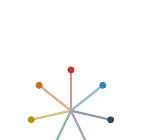
\begin{tikzpicture}[scale=0.45]
  \voicerose{0}{0}{1.15}{0.1}
\end{tikzpicture}
\end{minipage}
\end{center}
\vspace*{\fill}


\clearpage
% ============================= APPENDIX: THE OLD WHEEL =============================
\section*{Appendix. An old wheel under the optics}
\addcontentsline{toc}{section}{Appendix. An old wheel under the optics}

\noindent\emph{This case study stands outside the book's main road:
a worked example of the optics applied to a pre-scientific system of
self-description. It is included for one reason --- it shows, on a
hard case, how the honesty marks separate an instrument from a
story.}\medskip

% ============================= 14b. OLD INSTRUMENTS =============================

If a pattern can read itself, it will start doing so long before
theorems. For millennia people built \emph{instruments of
self-description}: the sixty-four hexagrams of the I~Ching are six
yes/no answers, exactly six bits; the starry sky is a shared clock
with hands of different slowness; wheels of birth, charts of
character. Before any science --- out of observation and a hunger
for self-reading. To throw them away is arrogance; to take them on
faith is credulity. The third way is to \emph{take them apart}.

We took apart one such wheel --- a modern fusion of the I~Ching with
the star clock --- down to the last screw, by machine check. Inside
there turned out to be three layers, and it matters not to confuse
them.

\textbf{Layer one: a real clock.} The wheel's computing machinery is
honest astronomy: planetary positions, a precise arc, careful
arithmetic. Here everything reproduces to the last digit (computed;
we even found a genuine bug in a popular calculation program --- and
the source book confirmed it against the code).

\textbf{Layer two: real but hidden combinatorics.} Mathematics is
hidden in the wheel that its own adepts do not know about. Opposite
gates of the wheel are \emph{exact binary complements}: all
thirty-two out of thirty-two (computed). The famous ``percentages of
human types'' are not empirics but the arithmetic of the
construction itself: you can obtain them without polling a single
person (computed). The whole system of ``profiles'' with its
canonical frequencies is the fractional part of \emph{one single
number}, $93.87$ (computed): an entire symbolic universe folds into
one line. Kepler signed the curve of the year: the Earth lingers at
the far point of its orbit, and the ``summer'' gates collect $3.4\%$
more births (computed exactly, from boundary-crossing times). And a
check against one hundred sixteen million real birth records showed:
the ``eternal type percentages'' are a portrait of the twentieth
century; slow planets park in gates for decades and hand them to
whole generations, so for those born after 2000 the distribution
must be different --- testable right now (computed).

\textbf{Layer three: the storyteller.} But the bridge from the wheel
to the fate of a concrete person is supported by nothing: no
mechanism of influence is presented, no correlations with real
people have been checked, and any future blind test must remember
that the most frequent ``type'' is guessed in two cases out of three
by pure arithmetic, with no sky at all. The meanings were written
into the wheel by a storyteller --- as they would be written into
any honest clock.

What this says about the world --- by UHM \stI. The longevity of
such systems is not the foolishness of ancestors but the
\emph{pattern's demand for self-reading}: symbolic systems are early
organs of self-description, drafts of that same questionnaire of
seven voices. And the boundary between instrument and superstition
runs not along the age of a system but along the honesty of its
marks: an instrument says what it measures and where its right
ends; superstition does not. By this --- by this alone --- the
present book differs from a horoscope.

\begin{figure}[H]
\centering
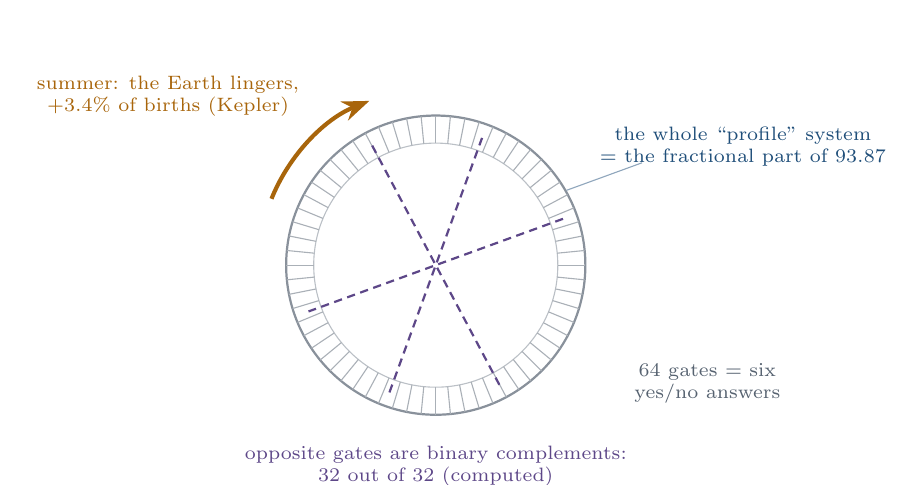
\begin{tikzpicture}[font=\small, >=Stealth]
  \draw[plosgray!70, thick] (0,0) circle (1.9);
  \draw[plosgray!40] (0,0) circle (1.55);
  \foreach \i in {0,...,63}{ \draw[plosgray!50] ({90-\i*5.625}:1.55) -- ({90-\i*5.625}:1.9); }
  \foreach \a in {20, 118, 250}{ \draw[dusk, thick, densely dashed] (\a:1.72) -- ({\a+180}:1.72); }
  \node[font=\scriptsize, text=dusk, align=center] at (0,-2.55)
    {opposite gates are binary complements:\\ 32 out of 32 (computed)};
  \draw[->, line width=1.5pt, ember] (158:2.25) arc (158:112:2.25);
  \node[font=\scriptsize, text=ember, align=center] at (-3.4,2.15)
    {summer: the Earth lingers,\\ $+3.4\%$ of births (Kepler)};
  \node[font=\scriptsize, text=fact, align=center] at (3.9,1.5)
    {the whole ``profile'' system\\ $=$ the fractional part of $93.87$};
  \draw[fact!50] (2.62,1.3) -- (1.66,0.95);
  \node[font=\scriptsize, text=plosgray, align=center] at (3.45,-1.5)
    {64 gates $=$ six\\ yes/no answers};
\end{tikzpicture}
\caption{A divination wheel under the microscope: an honest clock,
hidden binary combinatorics, Kepler's signature in the curve of the
year --- and over it all a storyteller whose bridge to a person's
fate is supported by nothing. Taking apart is more respectful than
either believing or laughing.}
\label{fig:wheel}
\end{figure}

\begin{talebox}[The campfire tale --- the wheel with a little mirror]
In one village stood a wheel: turn it, and it would tell your fate.
A craftsman came and took it apart. Inside were a clock --- real,
precise --- and a little mirror. ``It does not know fate,'' said the
craftsman. ``It honestly shows the sky and you. The fate was written
into it by storytellers.'' The village thought --- and did not throw
the wheel away. They began to measure by the clock, to look into the
mirror, and to tell their fate themselves.
\end{talebox}

\begin{askbox}[Ask yourself]
What ``wheels'' spin today --- personality tests, typologies,
calendars of luck? Take your favorite and find its three layers:
where is the honest clock, where the hidden mathematics, and where
the storyteller? What remains once the layers are labeled?
\end{askbox}


\end{document}
